\clearpage

\section{Result} 

\subsection{Statical Analysis and Hypothetical Test} \label{sec::Result::statistics}
\paragraph{The Profle Likelihood and Treatment of Systematics}
Statitical tests are performed to examine the consistency of observed data with respect to prediction of SM or that with specific signal being overlayed. This is implemented via a likelihood function based on the probability desnsity distribution (PDF) in terms of number of observed events in each signal region bin. The full representation of the likelihood is given by Eq. \ref{eq::Result::LH}:
\begin{align}
 \mathcal{L} (\mu; \muw, \mutop, \bmtheta)  
 & =  \mathcal{L} ( \bm{n}^{\SR}, \bm{n}^{\WR}, \bm{n}^{\TR} | \mu, \muw, \mutop, \bmtheta) \nn \\
  & = \mathcal{P}_{\SR} \times \mathcal{P}_{\CR}  \times \prod_{k\in \mathrm{syst.}} \rho(\theta_k), \\
& \nn \\
% 
  \mathcal{P}_{\SR} & = \prod_{i\notin \textbf{3B}} \,\, \left[ \prod_{b \in \mathrm{BT}, \mathrm{BV}} \,\, \mathrm{Pois}\, (n^{\SR}_{i,b} | \mu s^{\SR}_{i,b}(\bmtheta) + \muw \,  w^{\SR}_{i,b}(\bmtheta) + \mutop \,  t^{\SR}_{i,b}(\bmtheta) + b^{\SR}_{i,b}(\bmtheta)) \right] \nn \\
& \times \prod_{i\in \textbf{3B}} \,\, \mathrm{Pois}\, (n^{\SR}_i | \mu s^{\SR}_i(\bmtheta) + \muw \,  w^{\SR}_i(\bmtheta) + \mutop \,  t^{\SR}_i(\bmtheta) + b^{\SR}_i(\bmtheta))  \\
& \nn\\
%
  \mathcal{P}_{\CR} =  \prod_i \,\,
  &        \mathrm{Pois}\, (n^{\TR}_i | \mu s^{\WR}_i(\bmtheta) + \muw \,  w^{\WR}_i(\bmtheta) + \mutop \,  t^{\WR}_i(\bmtheta) + b^{\WR}_i(\bmtheta))  \nn \\
  & \times \mathrm{Pois}\, (n^{\WR}_i | \mu s^{\TR}_i(\bmtheta) + \muw \,  w^{\TR}_i(\bmtheta) + \mutop \,  t^{\TR}_i(\bmtheta) + b^{\TR}_i(\bmtheta))  
\label{eq::Result::LH}
\end{align}
where 
$\bm{n}^{\SR}$, $\bm{n}^{\WR}$ and $\bm{n}^{\TR}$ are respectively the numbers of observed events in SRs, corresponding CRs such as WRs and TRs, with the vetor indices running over ;
$s_{r}$ is the expected signal yield in region $r$ in the signal model to be tested;
$w_{r}$ and $t_{r}$ are respectively the expectated yields of $\wjets$ and $\ttbar$ in region $r$ before the normalization, with the components derived by the object replacement method being exluded;
$b_{r}$ are the expectated yields of the other backgrounds in region $r$;
$\bmtheta$ is the vector of nuisance parameters for each systematic uncertainty; 
$\muw$ and $\mutop$ are the normalization factors for $\wjets$ and $\ttbar$ which are allowed to vary between $i$; 
and $\mu$ is the signal strength, a parameter denoting relative normalization with respect to the signal model to be tested i.e. $\mu=0$ corresponds to a background-only hypothesis and $\mu=1$ to a hypothesis with the nominal signal level expected by the signal model. Index $i$ runs along signal region bins joining the combined fit that are orothgonal to each other s.t. :
%
\begin{align}
i \in \,\, \{ \,\,\, & \textbf{2J},\textbf{6J},\textbf{3B}  \,\,\, \}  \nn \\
\mbox{ or } & \{ \,\, \textbf{2J},\textbf{High-x},\textbf{3B} \,\,\}  \nn \\
\mbox{ or } & \{ \,\, \textbf{Low-x},\textbf{6J},\textbf{3B} \,\,\}  \nn \\
\mbox{ or } & \{ \,\, \textbf{Low-x},\textbf{High-x},\textbf{3B} \,\,\}
\end{align}
where
\begin{align}
\textbf{2J} & = \,\, \{ \,\,\, \mbox{2J-$\meffIncFirst$, 2J-$\meffIncSecond$, 2J-$\meffIncThird$}  \,\,\, \}  \nn \\
\textbf{6J} & = \,\, \{ \,\,\, \mbox{6J-$\meffIncFirst$, 6J-$\meffIncSecond$, 6J-$\meffIncThird$}  \,\,\, \}  \nn \\
\textbf{Low-x} & = \,\, \{ \,\,\, \mbox{Low-x}  \,\,\, \}  \nn \\
\textbf{High-x} & = \,\, \{ \,\,\,\mbox{High-x}   \,\,\, \}  \nn \\
\textbf{3B} & = \,\, \{ \,\,\, \mbox{3B-$\meffIncFirst$, 3B-$\meffIncSecond$}  \,\,\, \}  \nn \\
\end{align}

The normalization factors for $\wjets$ and $\ttbar$ backgrounds are simultaneouly determined by the fit,
in order to correlate the behavior of systematics.
Therefore the CRs terms are also placed in the common likelihood with an identical representation as SRs. \\

The statistical behavior of the PDF is fully characterized by a set of independent poisson PDF, namely:
\begin{align}
\mathrm{Pois}\,(n|\nu) & := \frac{\nu^n}{n!} e^{-\nu} \nn
\end{align}
with $\nu$ and $n$ being the expected yield and observed number repectively. \\

The effect of a systematics (indexed by $k$) are then incorporated by shifting the poisson means $\nu$, via a corresponding nuisance parameter $\theta_k$ so as:
\begin{align}
        \nu(\theta_k) := f(\theta_k), 
\end{align}
with $f(\theta_k)$ being a continuous function satisfying:
\begin{align}
        f(\theta_k=0) & =  \nu(0)  \nn \\
        f(\theta_k=\pm1) & =  \nu(\pm1\sigma).
\end{align}
$\nu(0)$ is the nominal expectation yields, while $\nu(\pm1\sigma)$ is given by that with the systematic variation applied by $\pm1\sigma$ which are evaluated beforehand. $f(\theta_k)$ in the other $\theta_k$ is then interporated or extrapolated using the three points by a polynomial or an exponential function, providing a continuous functional form of $\mathcal{L}$ in terms of $\bmtheta$.

What is here intend to do is to perform a global fit on data, simultaneously determining $\mu, \muw, \mutop$ and $\bmtheta$ by minimizing the likehood $\mathcal{L}$ (Eq. \ref{eq::Result::LH}). While the $\mu, \muw$ and $\mutop$ are allowed to flow based on our total ignorance, the shifts of the nuisance parameters $\bmtheta$ need to be restricted reflecting the level of our confidence. This is implemented by the last terms in the likelihood $\rho(\theta_k)$ known as the ``penalty terms'' serving as the prior constraints for the likehood. The form of the penalty terms depends on the statistical nature of each systematics:
\begin{itemize}
%jav. need to change
\item A Gaussian PDF is commonly assumed for most systematic uncertainties:
\begin{align}
%\rho (\theta) = \frac{1}{\sqrt{2\pi}\sigma} \mathrm{exp} \left( - \frac{(\theta-\hat{\theta})^2}{2\sigma^2} \right)
\rho (\theta) = \frac{1}{\sqrt{2\pi}\sigma} \mathrm{exp} \left( - \frac{\theta^2}{2} \right)
\end{align}

%\begin{align}
%\rho (\theta) = \frac{1}{\sqrt{2\pi}\log{\sigma}} \mathrm{exp} \left( - \frac{(\log{(\theta/\hat{\theta})})^2}{2(\log{\sigma})^2} \right) \frac{1}{\theta}
%\end{align}

\item The Gamma PDF is used to describe uncertainties following according to Poisson distribution, typically associated with the number of data events in control regions, or selected MC events:
\begin{align}
& \rho (a) = \frac{\nu^a}{a!} e^{-\nu} 
\end{align}
where $a$ is related with $\theta$ using the symmetrized uncertainty by 
\begin{align}
& \theta = \frac{a-\nu}{\sigma} \nn \\
\end{align}
\end{itemize}

A multi-dimensional minimization over the parameter spaces of all the normalization factors, nuisance parameters and signal strength 
\footnote{Remind that we have $8-16$ normalization factors and $\sim 150$ nuisance parameters in case of combined fit over all SR towers.}
is performed by the Minuit2 algorithm \cite{Minuite2} interfaced by a number wrapper packages; \texttt{HistFitter} \cite{HistFitter}, \texttt{HistFactory} \cite{HistFactory} and \texttt{RooFit} \cite{RooFit}.
Signal strength and the background normalization factors are allowed to range $0-5$, while nuisance parameters are to moved by $-5\sigma - 5\sigma$ during the fit. Typically, the deminsion of systematics resulting in tiny enough impact on the yields in the SRs/CRs region bins (evaluated by the Kolmogorov-Smirov test) are excluded from the fit so as to reduce the redundant steps of scan (``pruning'').


%%%%%%%%%%%%%%%%%%%%
\paragraph{Hypothetical Testing}
A hypothetical test against a hypothesis $H$ is done by examining the compatibility with observation, via p-value $p^\mu$.
P-value is commonly defined as the probability to find even rarer outcome than observation under $H$. 
For the simpleest one bin counting experiment, expecting an data excess as signal, it can be derived as:
\begin{align}
p_\mu := \sum_{n=n_{\mathrm{obs}}}^{\infty} L(n|\mu) 
\end{align}
using the number of observed events $n_{\mathrm{obs.}}$ as the test static.
One would claim a discovery against the null hypothesis $H_0$ if the $p_0$ is significantly low that the observation can be hardly ascribed to statistical fluctuation out of $H_0$. In the filed of high energy physics experiment, this is usually set to one corresponding to $5\sigma$ gaussian standard deviation ($\sim 10^{-7}$). \\

On the other hand, one can claim the exclusion of a signal hypothesis $H_1$ when $p_1$ is reasonably low. $p_1<0.05$ is conventionally used as the threshold, equivalent to an exclusion with $95\%$ confidence level. There are circumstates where observation does not agree with either $H_0$ and $H_1$ due to statistical fluctuation or more seriously poor understanding to backgrounds, and result in strong exclusion power typically when data undershoots the expectation. In LHC, in order to prevent such potentially unreasonably strong exclusion, a modified measure $cls$ is used:
\begin{align}
\cls := \frac{p_1}{1-p_0},
\end{align}
and $\cls<0.05$ is accepted as the equivalence of an exclusion at $95\%$ confidence level. \\

In presence of multiple test statics ($\bm{n}^{\SR}$) together with bunches of nuisance parameters, it is not obvious how to define the ``rareness'' on the muti-dimension of space. In such cases, likelihood is often chosen as the test static projecting n-dimension observables into 1 dimension, as well as providing a well-defined meausre of ``reareness'' by definition. In LHC analysis, a normalized likelihood test static $\lambda_\mu$ is widely used:
\begin{align}
\lambda_\mu = 
        \begin{cases}
        \dfrac{ \mathcal{L} (\mu, \hat{\hat{\bmtheta}}(\mu)) }{ \mathcal{L} (\hat{\mu}, \hat{\bmtheta})  }         \mbox{\phantom{MMMMMMMMMM}} (\hat{\mu}>0)        \\
        \dfrac{ \mathcal{L} (\mu, \hat{\hat{\bmtheta}}(\mu)) }{ \mathcal{L} (0, \hat{\hat{\bmtheta}}(0))  }  \mbox{\phantom{MMMMMMMMMM}} (\hat{\mu}<0)
        \end{cases}
\end{align}
where $\hat{\hat{\theta}}(\mu)$ denotes the best-fit nuisance parameters with fixed $\mu$,
while $\hat{\mu}$ and $\hat{\theta}$ the best-fit parameters with $\mu$ is allowed to float. 
$\mathcal{L} (\mu, \hat{\hat{\theta}}(\mu))$ presents the conditional likelihood normalized by the $\mu$-agonistic denominator $\mathcal{L} (\hat{\mu}, \hat{\theta})$, forcing the range of $\lambda_\mu$ to $0<\lambda_\mu<1$. \\
%(Eq. \ref{sec::Result::LH})

The p-value is finally defined as:
\begin{align}
p_\mu := \int_{q_{\mu,\mathrm{obs.}}}^{\infty}  f(q^{\mu}|\mu) dq_\mu
\end{align}
where $q_{\mu}$ is:
\begin{align}
q_{\mu} = 
        \begin{cases}
        -2 \log\lambda(\mu)     \,\,\,\,  (\hat{\mu} < \mu) \\
        \mbox{\phantom{k}} 0     \mbox{\phantom{MMMMM}} (\hat{\mu} > \mu)
        \end{cases}
\end{align}
and $f(q_\mu)$ is the PDF that $q_\mu$ obeys, defined by the vaiation of $q_\mu$ (1-to-1 to the variation on the best-fit likelihood value) when suffering from both the statistical fluctuation as well as systematics.
In principle this requires a bunch of toy experiments; scanning from $\mu=0$ upto $\mu=5\sim 10$ with a finite step, on each of which a number of the likelihood fits are performed with different fluctuating data statistics and systematic variation applied. This is an incredibly crazy course of computation.
\footnote{Each likehood fit takes typically 8-12 minutes. }

Fortunately, there are a couple of powerful approximation formula; Wald's approximation:
\begin{align}
q_\mu = -2 \log\lambda(\mu) = \frac{\mu-\hat{\mu}}{\sigma^2} + O(1/\sqrt{N})
\end{align}
and the Asimov's asymptotic formula using the result above:
\begin{align}
f(q_\mu,\mu) & = \frac{1}{\sqrt{q_\mu}} \frac{1}{\sqrt{2\pi}} \left[ \exp \left( -\frac{1}{2}(\sqrt{q_\mu}+\sqrt{R}) \right) + \exp \left( -\frac{1}{2}(\sqrt{q_\mu}-\sqrt{R}) \right) \right], \nn \\
R & := \frac{(\mu-\hat{\mu})^2}{\sigma^2},
\label{eq::asimov}
\end{align}
where $\sigma$ is the fitting error on $\hat{\mu}$ and $N$ symbolizes the magnitude of number of events in signal regions, with which the PDF $f(q_\mu)$ can be determined by only one fit.

One disclaimer is however about the validity of the approximation where $O(1/\sqrt{N})$ terms are ignored.
This may not be the case given that the signal regions typically contains events less than 5.
In the thesis, the result for background-only hypothesis (shown in Sec. \ref{sed::Result::bgOnly}) is derived using the rigid toy experiments, however the Asimov's formula (Eq.\ref{eq::asimov}) is nevertheless used for limit setting due to the unrealistic computing time required for the toy experiments. 
%Though it is generally claimed that the p-value could change, this would not change the grand picture of the resultant limits, given that rapid decrease of cross-section .
\footnote{This is in fact how ATLAS/CMS provides the result. We have to admit the imperfection but this is the best thing we could afford to do.}


\clearpage
\subsection{Unblinded Signal Regions with Background-only Hypothesis} \label{sed::Result::bgOnly}
The background expectation in signal regions for null singal hypothesis are determined tower-by-tower, 
by performing a simoultaneous fit on the normalization factors ($\mu_W$, $\mu_{\mathrm{Top}}$) as well as the nuisance parameters associated to systematics uncertainties, 
using all the relevent bins of control regions and signal regions.
The post-fit uncertainties are summarized in Fig. \ref{fig::Result::systSummary}.  \\

For the low $\meffInc$-bins, typically the estimation precision is at $20\%$ level where theory systematics is the main souce.
The signal region bins with tightest selection end up in $40\% \sim 60\%$ of total uncertainty, dominated by the control region statistics in the object replacement method. \\

The unblinded yields of observed data together with the expected backgrounds in the signal regions are shown in Tab. \ref{tab::Result::yieldsSRs_2J_6J} - \ref{tab::Result::yieldsSRs_3B}. Observed data are found to be consistent in general, with no signal regions exhibiting the deviation more than 2$\sigma$.
%A couple of minor excesses are found in some bins in the SR2JBV tower and SRHigh-xBT, however 
The pulls between data and expectation is shown in Fig. \ref{fig::Result::SRPulls}.

%%%%%%%%%%%%%%% SR Yields %%%%%%%%%%%%%%%%%%%%
\begin{table}
  \begin{center}
    \caption{
        Observed yields and backgrounds expection in the signal region bins in tower \textbf{2J} and \textbf{6J}.
        Background component estimated by the object replacement are denoted as ``Di-leptonic'', 
        while the others are derived from the kinematical extrapolation method. Displayed errors are only systematics uncertainty.
    \label{tab::Result::yieldsSRs_2J_6J}}
    \begin{tabular*}{\textwidth}{@{\extracolsep{\fill}}lrrrr}
\toprule
\textbf{SR 2J} $b$-tag & $m_{\mathrm{eff.}}\in$[1100,1500] & $m_{\mathrm{eff.}}\in$[1500,1900] & $m_{\mathrm{eff.}}>1900$ \\
\midrule

Observed data          & $8$              & $2$              & $1$                    \\
\midrule
Expected background         & $7.20 \pm 1.40$          & $2.46 \pm 0.60$          & $2.31 \pm 0.77$              \\
\midrule
        Di-leptonic         & $2.4 \pm 1.0$          & $0.8 \pm 0.4$          & $1.7 \pm 0.7$              \\
        $W$+jets         & $1.0 \pm 0.5$          & $0.1_{-0.1}^{+0.2}$          & $0.0 \pm 0.0$              \\
        $Z$+jets         & $0.6 \pm 0.2$          & $0.2 \pm 0.0$          & $0.1 \pm 0.0$              \\
        Tops         & $2.1 \pm 0.7$          & $0.8 \pm 0.3$          & $0.4 \pm 0.2$              \\
        Di-boson         & $0.4 \pm 0.1$          & $0.2 \pm 0.2$          & $0.1 \pm 0.0$              \\
        $t\bar{t}+V$         & $0.8 \pm 0.2$          & $0.3 \pm 0.1$          & $0.1 \pm 0.0$              \\
\toprule
\textbf{SR 2J} $b$-veto & $m_{\mathrm{eff.}}\in$[1100,1500] & $m_{\mathrm{eff.}}\in$[1500,1900] & $m_{\mathrm{eff.}}>1900$ \\
\midrule
Observed data          & $25$              & $8$              & $6$                    \\
\midrule
Expected background         & $13.33 \pm 2.59$          & $6.84 \pm 1.44$          & $2.53 \pm 0.66$              \\
\midrule
        Di-leptonic         & $2.4 \pm 1.8$          & $2.3 \pm 1.1$          & $0.7 \pm 0.6$              \\
        $W$+jets         & $4.2 \pm 1.1$          & $1.6 \pm 0.4$          & $0.4 \pm 0.2$              \\
        $Z$+jets         & $2.3 \pm 0.7$          & $1.0 \pm 0.3$          & $0.6 \pm 0.2$              \\
        Tops         & $1.1 \pm 0.4$          & $0.3 \pm 0.1$          & $0.2 \pm 0.1$              \\
        Di-boson         & $3.2 \pm 1.1$          & $1.6 \pm 0.5$          & $0.7 \pm 0.2$              \\
        $t\bar{t}+V$         & $0.1 \pm 0.0$          & $0.1 \pm 0.0$          & $0.0 \pm 0.0$              \\


\bottomrule
%%
\end{tabular*}





    \begin{tabular*}{\textwidth}{@{\extracolsep{\fill}}lrrrr}
\toprule
\textbf{SR 6J} $b$-tag &  $m_{\mathrm{eff.}}\in$[1100,1600] & $m_{\mathrm{eff.}}\in$[1600,2100] & $m_{\mathrm{eff.}}>2100$ \\
\midrule

Observed data          & $7$              & $3$              & $0$                    \\
\midrule
Expected background         & $5.09 \pm 1.04$          & $2.14 \pm 0.65$          & $2.46 \pm 0.89$              \\
\midrule
        Di-leptonic         & $2.6 \pm 0.8$          & $1.1 \pm 0.6$          & $1.5 \pm 0.8$              \\
        $W$+jets         & $0.4 \pm 0.2$          & $0.1 \pm 0.1$          & $0.1 \pm 0.1$              \\
        $Z$+jets         & $0.0_{-0.0}^{+0.0}$          & $0.0 \pm 0.0$          & $0.0_{-0.0}^{+0.0}$              \\
        Tops         & $1.0 \pm 0.4$          & $0.5 \pm 0.2$          & $0.6 \pm 0.3$              \\
        Di-boson         & $0.2 \pm 0.1$          & $0.1 \pm 0.1$          & $0.1_{-0.1}^{+0.1}$              \\
        $t\bar{t}+V$         & $0.8 \pm 0.2$          & $0.3 \pm 0.1$          & $0.1 \pm 0.0$              \\
\toprule
\textbf{SR 6J} $b$-veto &  $m_{\mathrm{eff.}}\in$[1100,1600] & $m_{\mathrm{eff.}}\in$[1600,2100] & $m_{\mathrm{eff.}}>2100$ \\
\midrule
Observed data          & $5$              & $0$              & $1$                    \\
\midrule
Expected background         & $3.93 \pm 0.88$          & $1.28 \pm 0.36$          & $0.65 \pm 0.18$              \\
\midrule
        Di-leptonic         & $1.5 \pm 0.6$          & $0.2_{-0.2}^{+0.2}$          & $0.0 \pm 0.0$              \\
        $W$+jets         & $1.1 \pm 0.5$          & $0.6 \pm 0.3$          & $0.3 \pm 0.1$              \\
        $Z$+jets         & $0.2 \pm 0.1$          & $0.0 \pm 0.0$          & $0.0 \pm 0.0$              \\
        Tops         & $0.3 \pm 0.1$          & $0.1 \pm 0.1$          & $0.1 \pm 0.1$              \\
        Di-boson         & $0.7 \pm 0.2$          & $0.3 \pm 0.1$          & $0.2 \pm 0.1$              \\
        $t\bar{t}+V$         & $0.1 \pm 0.0$          & $0.0 \pm 0.0$          & $0.0 \pm 0.0$              \\


\bottomrule
%%
\end{tabular*}





  \end{center}
\end{table}

\begin{table}
  \begin{center}
    \caption{
        Observed yields and backgrounds expection in the signal region bins in tower \textbf{Low-x} and \textbf{High-x}.
        Background component estimated by the object replacement are denoted as ``Di-leptonic'', 
        while the others are derived from the kinematical extrapolation method. Displayed errors are only systematics uncertainty.
    \label{tab::Result::yieldsSRs_Lowx_Highx}}
    \begin{tabular*}{\textwidth}{@{\extracolsep{\fill}}lrrr}
\toprule
\textbf{SR Low-x} & $b$-tag &  $b$-veto \\
\midrule

Observed data & $0$ & $3$ \\
\midrule
Expected background & $2.04 \pm 0.70$ & $1.46 \pm 0.59$ \\
\midrule
Di-leptonic & $1.2 \pm 0.7$ & $0.6 \pm 0.5$ \\
$W$+jets & $0.1 \pm 0.0$ & $0.2 \pm 0.1$ \\
$Z$+jets & $0.0 \pm 0.0$ & $0.1 \pm 0.0$ \\
Tops & $0.6 \pm 0.2$ & $0.4 \pm 0.2$ \\
Di-boson & $0.1 \pm 0.0$ & $0.2 \pm 0.1$ \\
$t\bar{t}+V$ & $0.1 \pm 0.0$ & $0.0 \pm 0.0$ \\


\bottomrule
%%
\end{tabular*}





    \begin{tabular*}{\textwidth}{@{\extracolsep{\fill}}lrrr}
\toprule
\textbf{SR High-x} & $b$-tag & $b$-veto \\
\midrule

Observed data & $6$ & $4$ \\
\midrule
Expected background & $2.35 \pm 0.59$ & $4.27 \pm 0.94$ \\
\midrule
Di-leptonic & $0.8 \pm 0.5$ & $0.8 \pm 0.5$ \\
$W$+jets & $0.3 \pm 0.1$ & $1.7 \pm 0.5$ \\
$Z$+jets & $0.0_{-0.0}^{+0.0}$ & $0.5 \pm 0.2$ \\
Tops & $0.5 \pm 0.2$ & $0.1 \pm 0.1$ \\
Di-boson & $0.4 \pm 0.2$ & $1.1 \pm 0.5$ \\
$t\bar{t}+V$ & $0.3 \pm 0.1$ & $0.1 \pm 0.0$ \\


\bottomrule
%%
\end{tabular*}





  \end{center}
\end{table}

\begin{table}
  \begin{center}
    \caption{
        Observed yields and backgrounds expection in the signal region bins in tower \textbf{3B}.
        Background component estimated by the object replacement are denoted as ``Di-leptonic'', 
        while the others are derived from the kinematical extrapolation method. Displayed errors are only systematics uncertainty.
    \label{tab::Result::yieldsSRs_3B}}
    \begin{tabular*}{\textwidth}{@{\extracolsep{\fill}}lrrr}
\toprule
\textbf{SR 3B} & $m_{\mathrm{eff.}}\in$[1000,1750] & $m_{\mathrm{eff.}}>1750$ \\
\midrule
Observed data          & $2$              & $1$                    \\
\midrule
Expected background         & $2.06 \pm 0.68$          & $1.00 \pm 0.52$              \\
\midrule
        Di-leptonic         & $1.3 \pm 0.5$          & $0.8 \pm 0.5$              \\
        $W$+jets         & $0.0 \pm 0.0$          & $0.0 \pm 0.0$              \\
        $Z$+jets         & $0.0 \pm 0.0$          & $0.0 \pm 0.0$              \\
        Tops         & $0.6 \pm 0.4$          & $0.2 \pm 0.1$              \\
        Di-boson         & $0.0 \pm 0.0$          & $0.0 \pm 0.0$              \\
        $t\bar{t}+V$         & $0.2 \pm 0.1$          & $0.1 \pm 0.0$              \\


\bottomrule
%%
\end{tabular*}





  \end{center}
\end{table}


%%%%%%% Summary of post fit uncertainties %%%%%%%%%%%%%%%%
\fig[170]{Result/systSummary/syst_summary_SRs.pdf}
{
    Post-fit systematic uncertainty with respective to the expected yield in the signal regions. 
    Total systematics uncertainty is shown by the filled orange histogram, and the breakdowns are by dashed lines.
    While the systematics in b-tagged bins are purely dominated by control region statistics, 
    it is comparable to the other sources in the b-veto bins. The overall uncertainty ranges between $20\%\sim\%50$.
}       
{fig::Result::systSummary}
%-------------------------------                                                                                                                                                                                                                           
    
%%%%%%%%%%%%%%%%% SRpulls %%%%%%%%%%%%%%%%%%%%%%%%%%%%%%%%%%%%%%%
\fig[170]{BGestimation/PullVRsSRs/histpull_SRs.pdf}
{
    (Top) Observed yields and the background expectation in signal regions. The white component is the backgounds estimated by the object replacement method, while the colored ones are by the kinamtical extrapolation method. The dashed band represents the combined statistical and systematic uncertainty on the total estimated backgrounds.
    (Bottom) Pull between the observed data and the expectation. No significant deviation from expectation exceeding $2\sigma$.
}
{fig::Result::SRPulls}
%-------------------------------                                                                                                   

                                                                                                                         
\clearpage
\subsection{Constraints on the Benchmark Models}
The observed results are then interpretated into constraints on the benchamark models listed in Tab. \ref{tab::Introduction::modelsBV} - \ref{tab::Introduction::models3B}. The limits on the reference models (colored in Tab. \ref{tab::Introduction::modelsBV} - \ref{tab::Introduction::models3B}) are mainly presented in this section, while the full numerical results on the others models are shown in the Appendix. \\


\subsubsection{Exclusion Limits}
Fig. \ref{fig::Result::exclLimit::GG_onestepCC} presents the exclusion limit on QQC1QQC1, the reference model for BV benchmarks (Tab. \ref{tab::Introduction::modelsBV}). Hypothetical tests are done with each signal point using the combination of signal regions that gives the best expected sensitivity. The excluded region is defined by areas with $CL_s<0.05$, corresponding to $95\%$ confidence level. The associated expected limit is represented by a yellow band, showing the range of obtained limit if observed data is consistent to the expectation within $\pm1\sigma$. Observed limits are typically worse than the expected ones in the mass region where sensitivity is primarily driven by SR \textbf{2J} and SR \textbf{High-x}, namely the diagonal region in the \xhalf grid, and the high-$x$ region in the \varx grid respectively, reflecting the observed excess there which weakens the exclusion power. For the \xhalf and the \varx grid, limits are compared with the up-to-date published result provided by ATLAS \cite{strong1L_ICHEP2016_CONF}, shown as grey shades. The exclusion limits are pushed forward by about $200\gev\sim300\gev$ in gluino mass. Obviously, this owes a lot to the increased data statistics by factor of 2.5 though, the benefit by the improved analysis can also be acknowledged, given that the cross-section of gluino pair production falls more rapidly with respect the gluino mass increase, which is roughly $1/3$ by every $100\gev$.Upto $2\tev$ of gluino mass is excluted at the most optimistic massless LSP scenario, while it also reaches about $1.9\tev$ of gluino mass for the more realistic case with $0<\mLSP<1\tev$. 
% 
The constraints on the scenario where EW-gauginos are compressed, 
represented by the \DMth, \DMtw grids,
are explicitly investigated for the first time, which will provide useful input for a number of dark matter oriented SUSY phenomelogical models, such as the well-tempered neutrino scenario.
Though the limit is weaker than the typical signatures in \xhalf and \varx, sensitivity is addressed without loopholes. \\

Likewise, Fig. \ref{fig::Result::exclLimit::GG_QQC1BTC1} exhibits the limits for model QQC1BTC1, the reference model for BT benchmarks (Tab. \ref{tab::Introduction::modelsBV}). As the sensitivity is mainly driven by the b-tagged bins for this model, it is relatively more affected by the $\sim 1.9\sigma$ excess observed in the SR High-x BT, which drastically weakens the limit in the \varx grid. Nevertheless, the overall exclusion reach is comparable to QQC1QQC1, amounting to $1.9\sim2\tev$ in gluino mass for $\mLSP <1\tev$. As the the asymmetric decays of gluino have never been interpretated before, this is the first explicit constrains on such class of models. \\

The exclusion limit for the model TT11TTN1, the reference model for the 3B benchmarks (Tab. \ref{tab::Introduction::modelsBV}) is shown in Fig. \ref{fig::Result::exclLimit::GG_ttn1}. The observed and expected limits agree as the global feature. The most prominent update from the past result \cite{strong3B_ICHEP2016_CONF} by ATLAS (shaded area in the plot) is around the diagonal region with the mass spliting $\dmg$ below $400\gev$, where the explicit limit is set for the first time. On the other hand, there is seemingly no improvedment in the direction toward high gluino mass despite the increased data, which is because the compared limit is provided by the combination of both 0-lepton and 1-lepton channel in the analysis. The sensitivities driven by 1-lepton channel are compareable between the analyses. \\
%%%%%%%%
\clearpage
%% --
\begin{figure}[h]
  \centering
%    \subfigure[]{\includegraphics[width=0.48\textwidth]{figures/Result/exclContour/atlascls_wband1_wfixSigXSecband1_showcms0_myAna_tag858_objRep_shapeSys_excl_GG_onestepCC_fixSigXSecNominal_x12_hypotest__1_harvest_list.pdf}}
%    \subfigure[]{\includegraphics[width=0.48\textwidth]{figures/Result/exclContour/atlascls_wband1_wfixSigXSecband1_showcms0_myAna_tag858_objRep_shapeSys_excl_GG_onestepCC_fixSigXSecNominal_varx_hypotest__1_harvest_list.pdf}}
    \subfigure[]{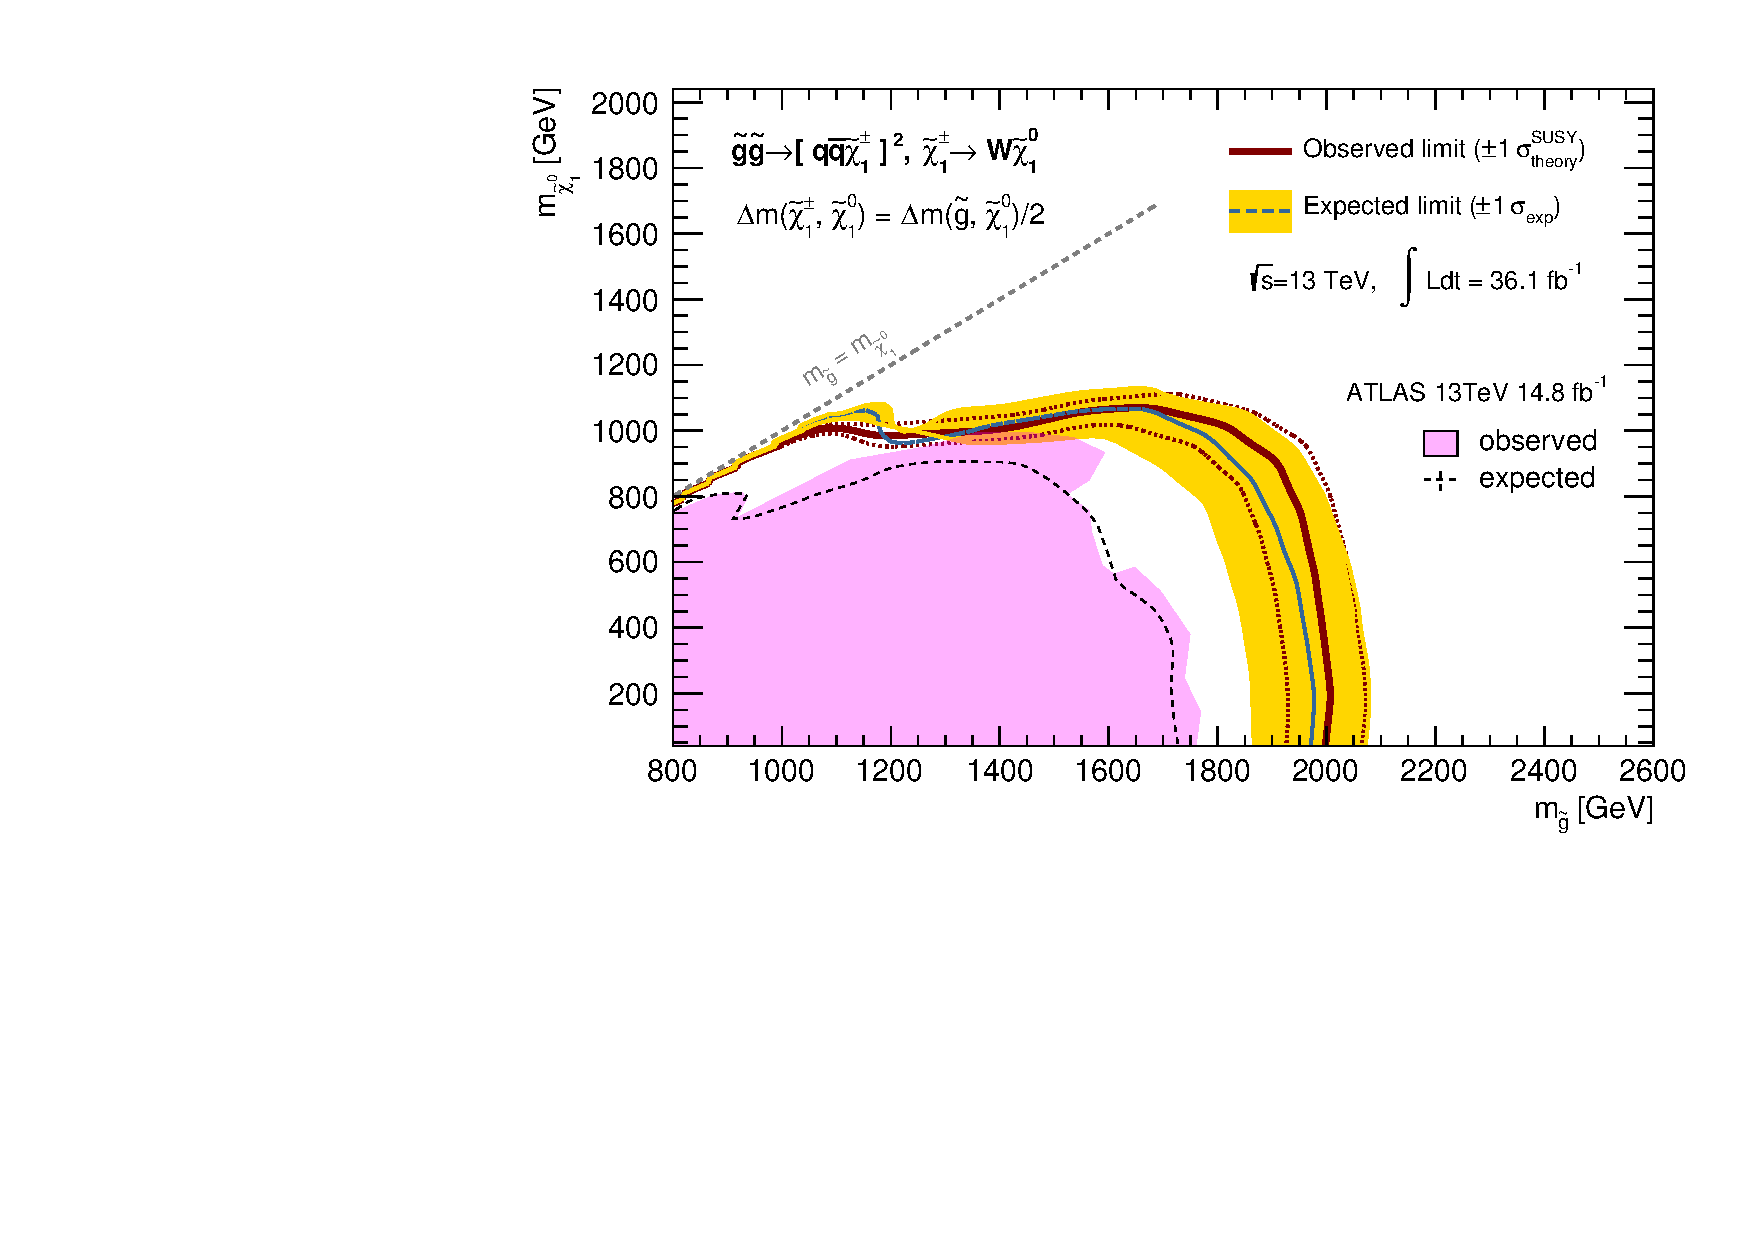
\includegraphics[width=0.48\textwidth]{figures/Result/exclContour/atlascls_wband1_wfixSigXSecband1_showcms0_myAna_tag858_objRep_shapeSys_excl_GG_symQQC1_fixSigXSecNominal_x12_hypotest__1_harvest_list.pdf}}
    \subfigure[]{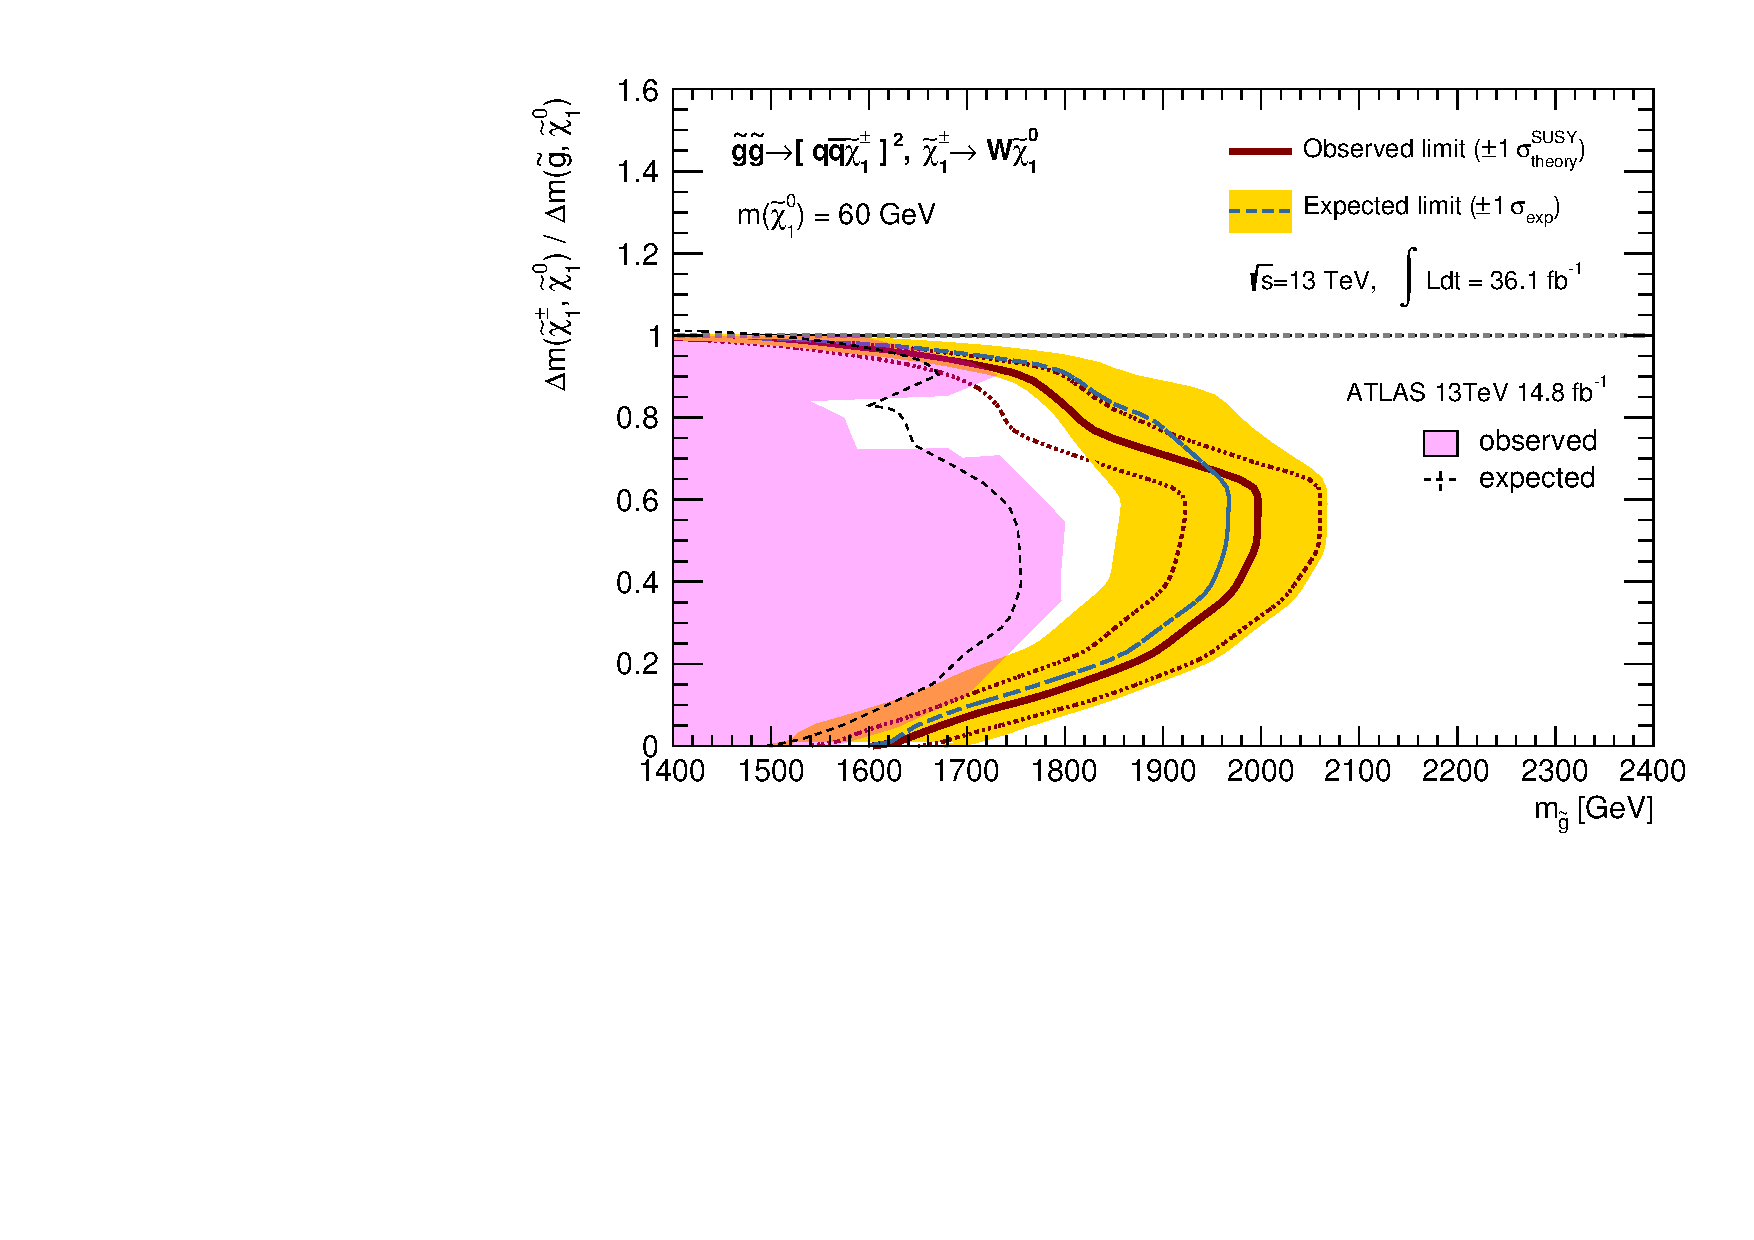
\includegraphics[width=0.48\textwidth]{figures/Result/exclContour/atlascls_wband1_wfixSigXSecband1_showcms0_myAna_tag858_objRep_shapeSys_excl_GG_symQQC1_fixSigXSecNominal_varx_hypotest__1_harvest_list.pdf}}
    \subfigure[]{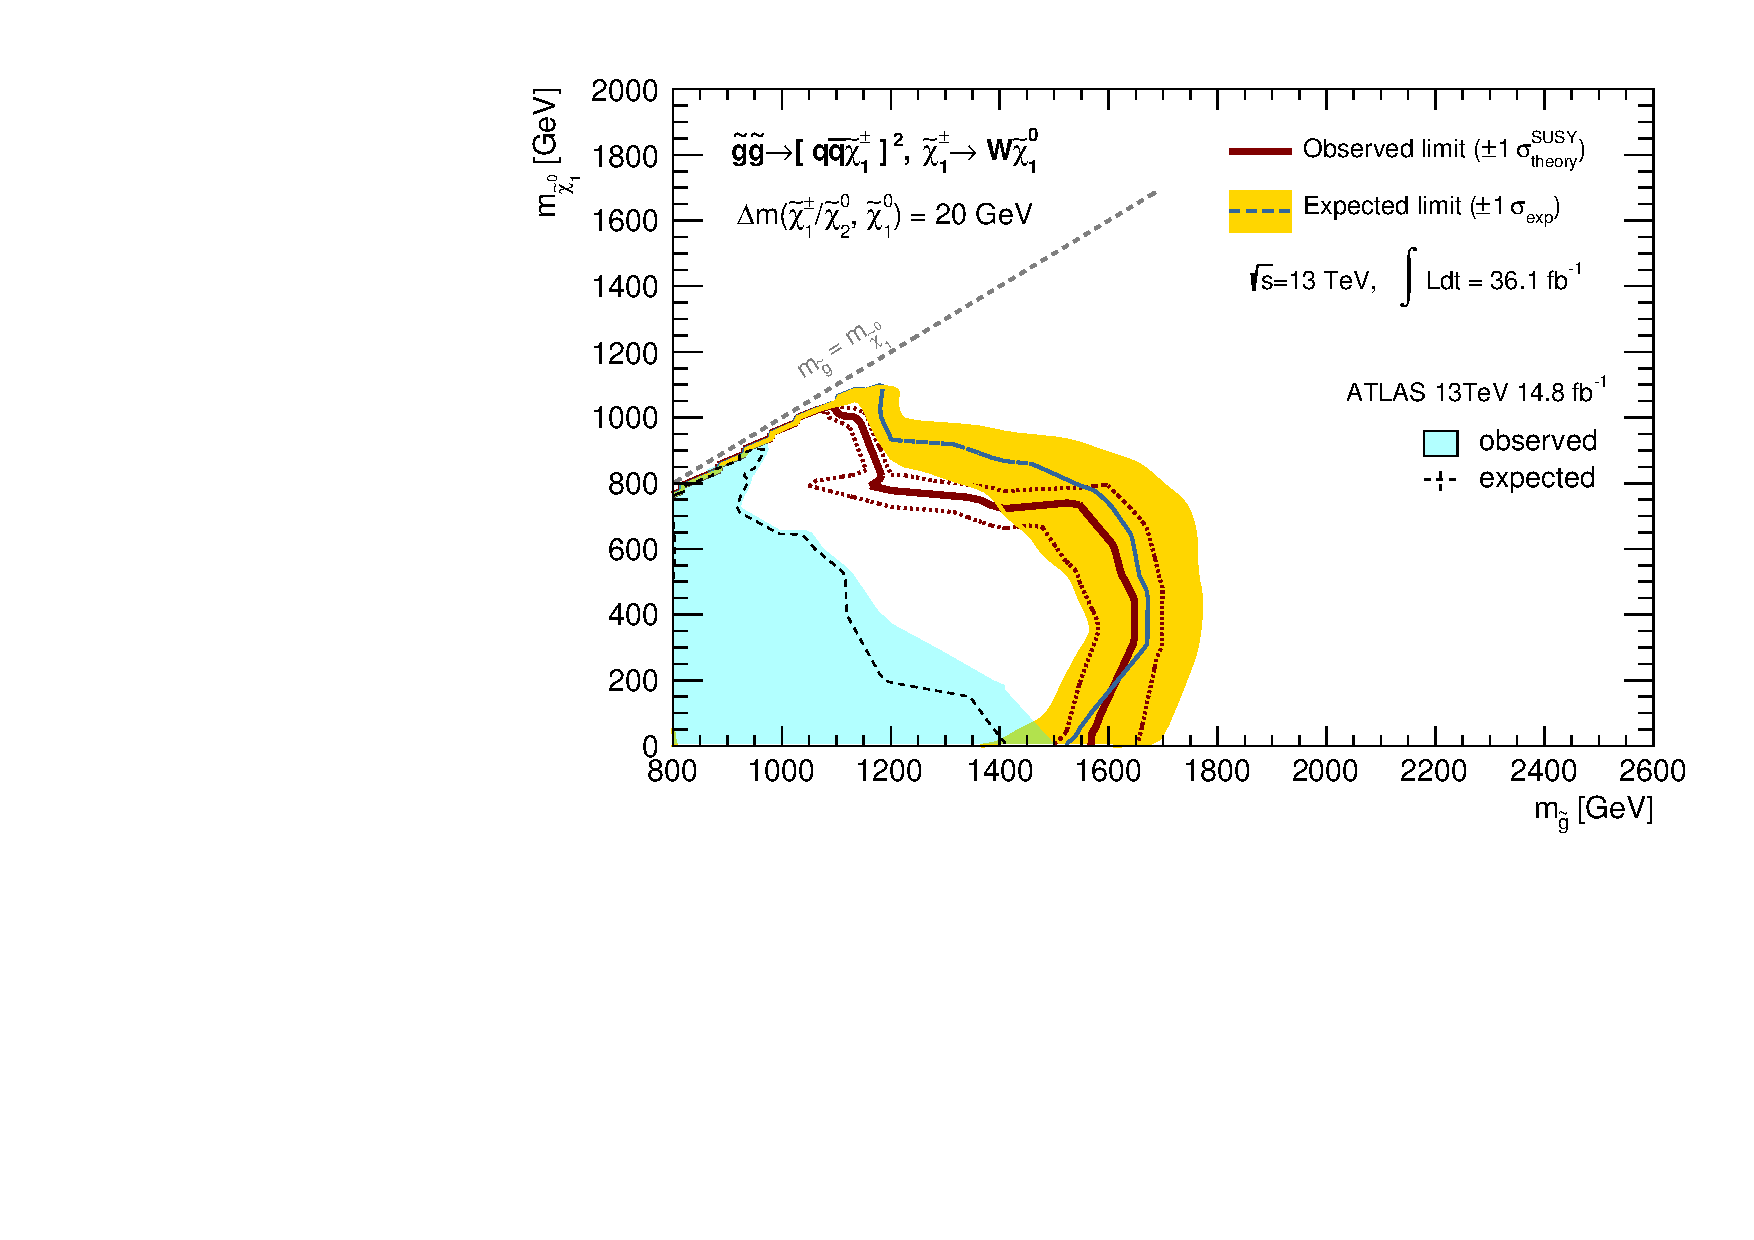
\includegraphics[width=0.48\textwidth]{figures/Result/exclContour/atlascls_wband1_wfixSigXSecband1_showcms0_myAna_tag858_objRep_shapeSys_excl_GG_symQQC1_fixSigXSecNominal_dM20_hypotest__1_harvest_list.pdf}}
    \subfigure[]{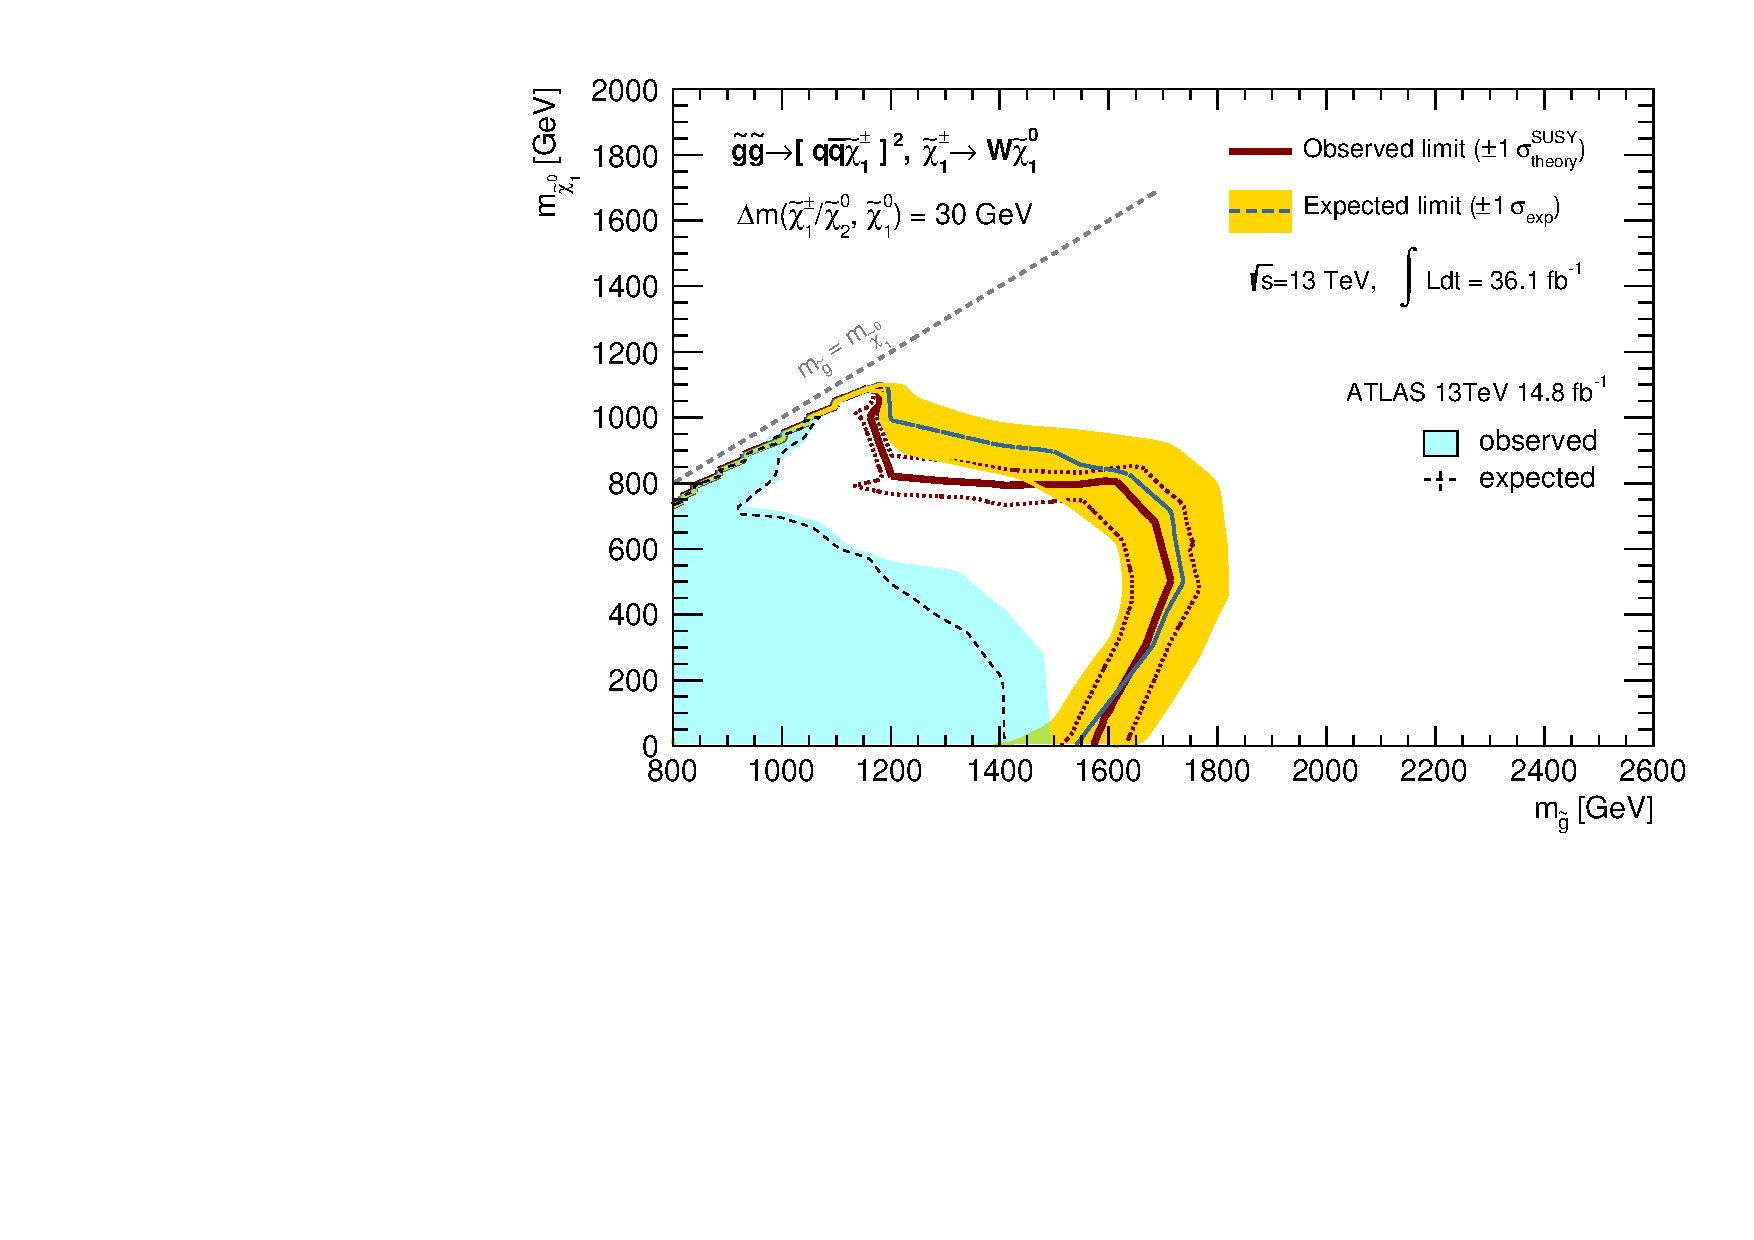
\includegraphics[width=0.48\textwidth]{figures/Result/exclContour/atlascls_wband1_wfixSigXSecband1_showcms0_myAna_tag858_objRep_shapeSys_excl_GG_symQQC1_fixSigXSecNominal_dM30_hypotest__1_harvest_list.pdf}}
    \caption{Exlusion limit for the benchmark model \textbf{QQC1QQC1} presented in the (a) \xhalf (b) \varx (c) \DMtw (d) \DMth grids. Observed limit is shown by the solid red line, while the expected limit are expressed by the dashed blue line with the yellow band describing the variation due to the deviation within $\pm1\sigma$. The up-to-date published result provided by ATLAS \cite{strong1L_ICHEP2016_CONF} is overlaid (observed limit: grey shade, expected limit: black dashed line). All limits correspond to 95$\%$ CL.
  \label{fig::Result::exclLimit::GG_onestepCC} }

\end{figure}


%figures/Result/exclContour/atlascls_wband1_wfixSigXSecband1_showcms0_myAna_tag858_objRep_shapeSys_excl_GG_symQQC1_fixSigXSecNominal_dM20_hypotest__1_harvest_list.pdf

%% --
\begin{figure}[h]
  \centering
    \subfigure[]{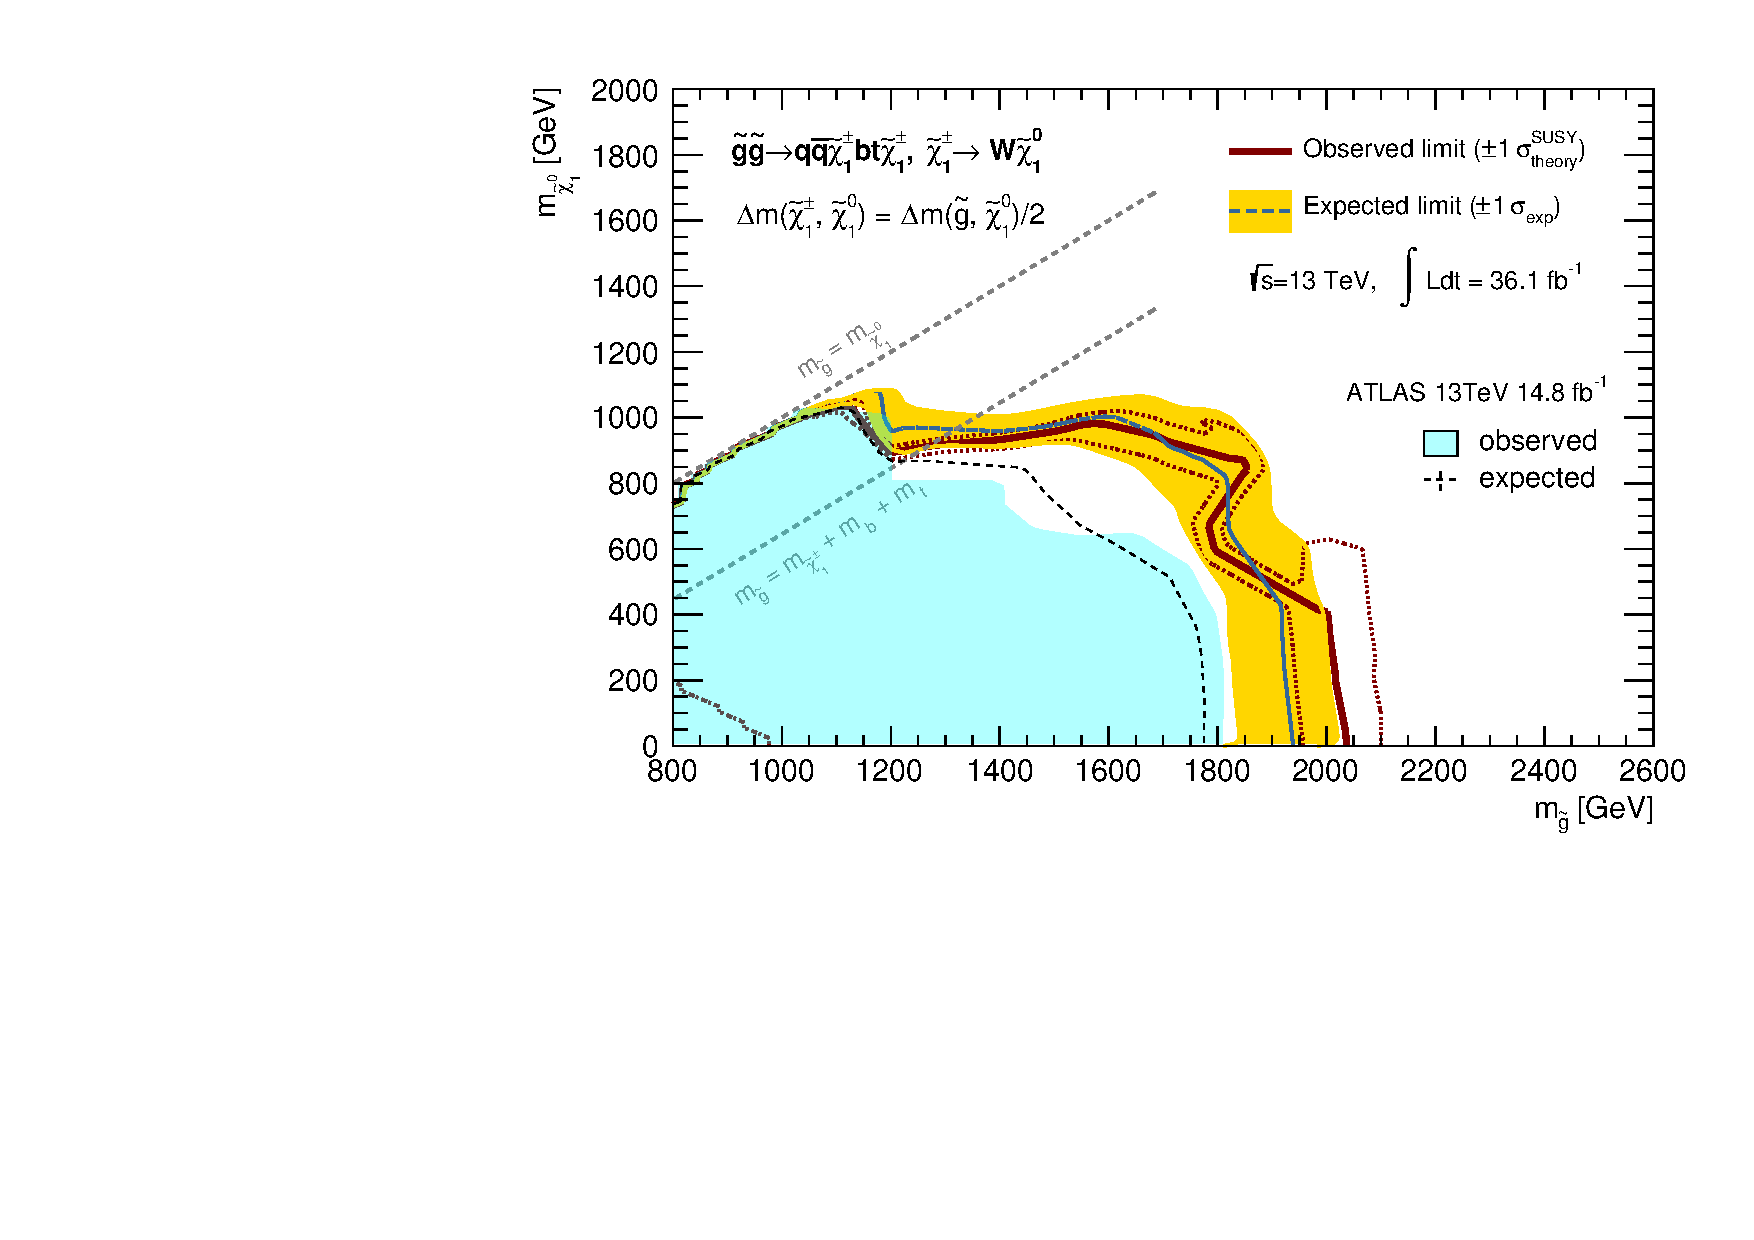
\includegraphics[width=0.48\textwidth]{figures/Result/exclContour/atlascls_wband1_wfixSigXSecband1_showcms0_myAna_tag858_objRep_shapeSys_excl_GG_QQC1BTC1_fixSigXSecNominal_x12_hypotest__1_harvest_list.pdf}}
    \subfigure[]{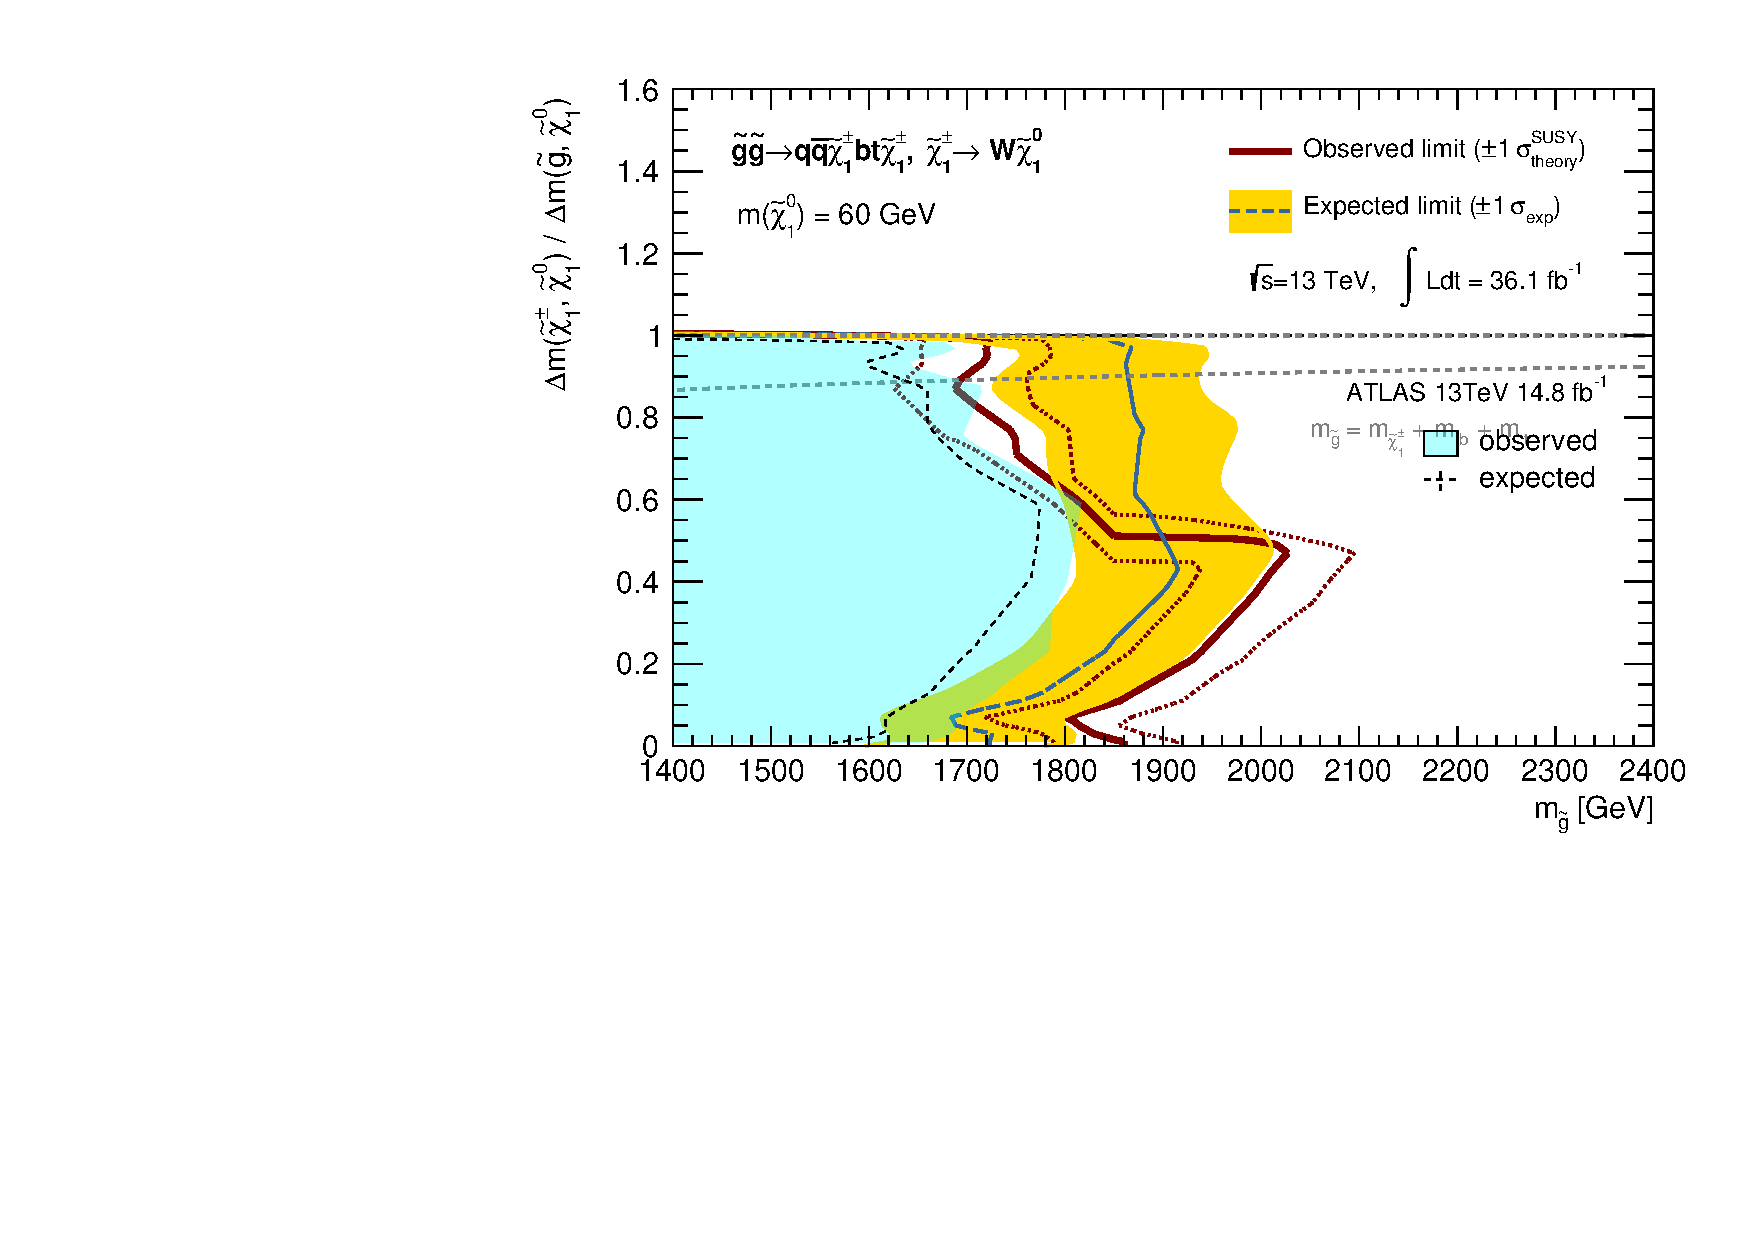
\includegraphics[width=0.48\textwidth]{figures/Result/exclContour/atlascls_wband1_wfixSigXSecband1_showcms0_myAna_tag858_objRep_shapeSys_excl_GG_QQC1BTC1_fixSigXSecNominal_varx_hypotest__1_harvest_list.pdf}}
    \subfigure[]{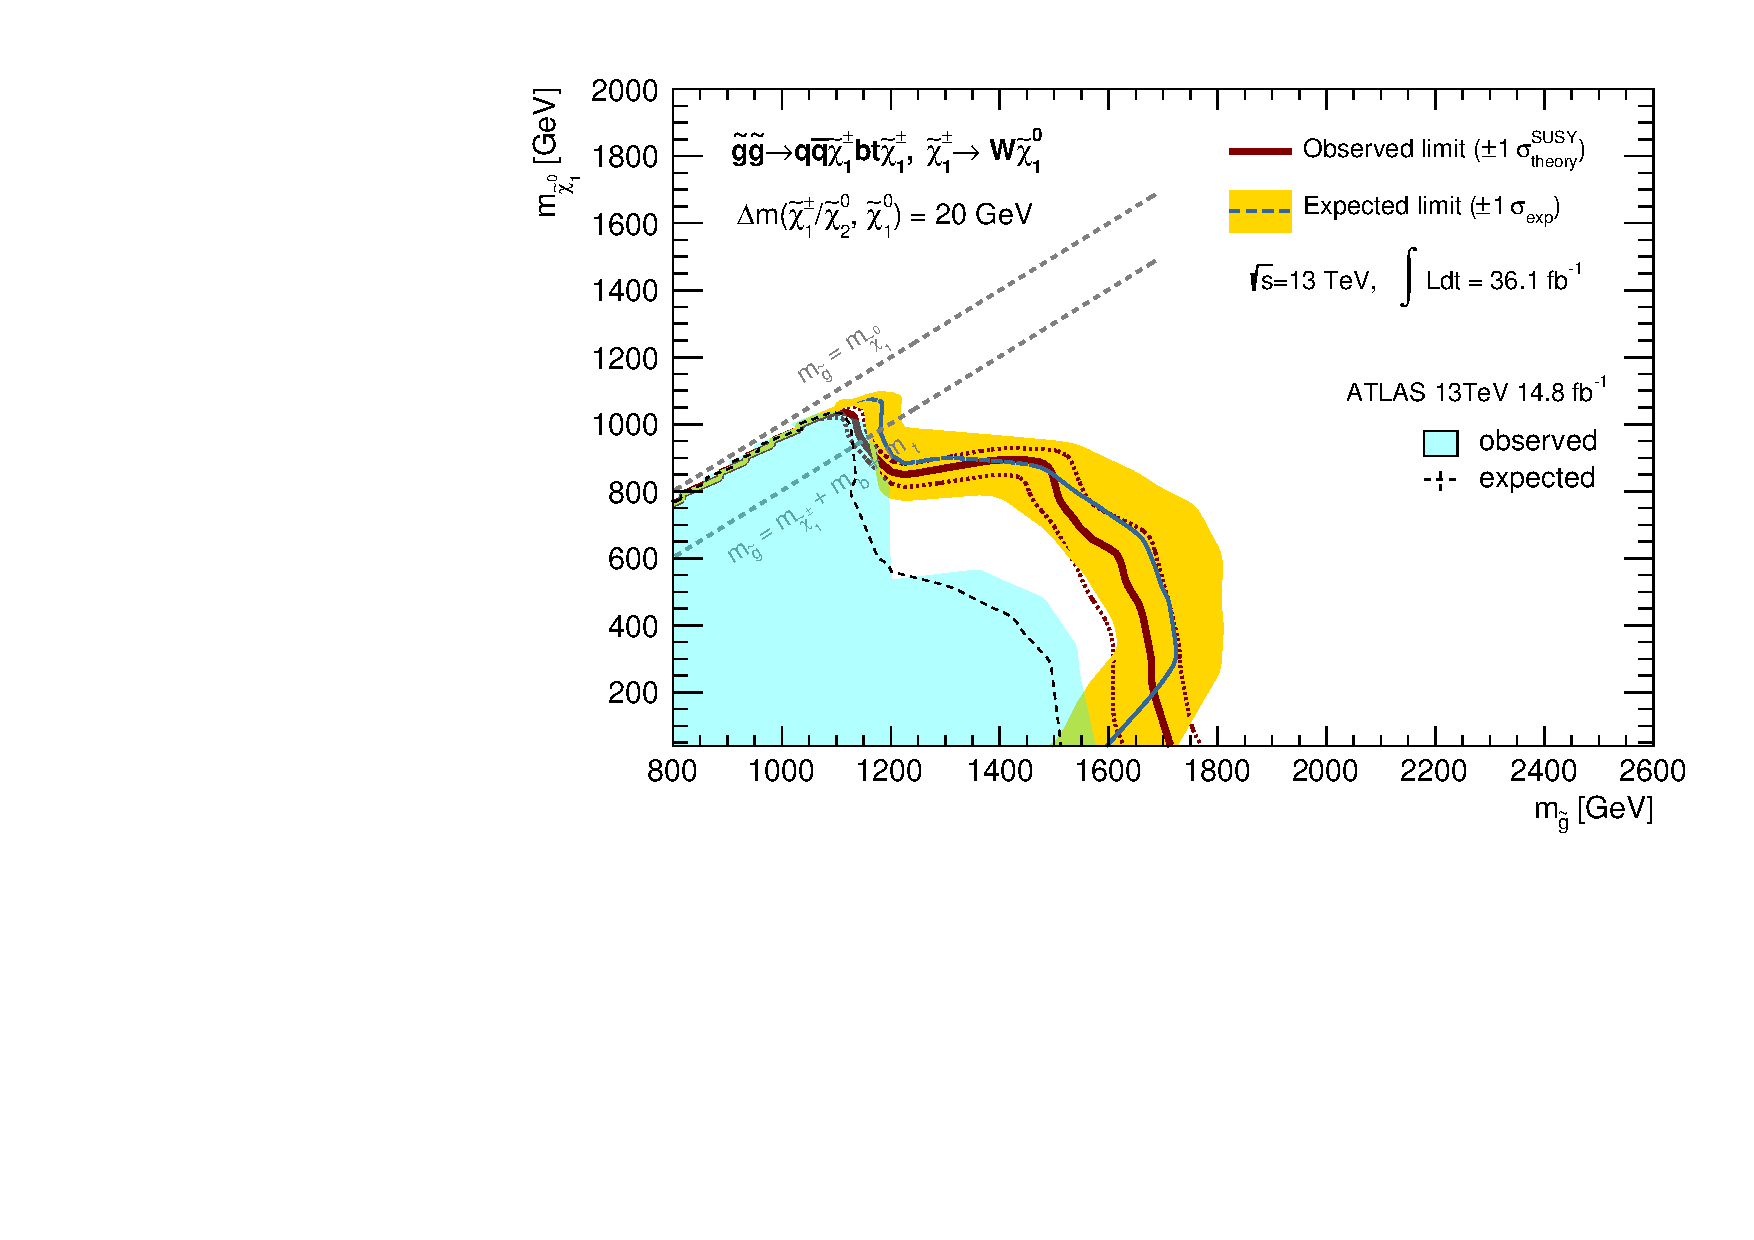
\includegraphics[width=0.48\textwidth]{figures/Result/exclContour/atlascls_wband1_wfixSigXSecband1_showcms0_myAna_tag858_objRep_shapeSys_excl_GG_QQC1BTC1_fixSigXSecNominal_dM20_hypotest__1_harvest_list.pdf}}
    \subfigure[]{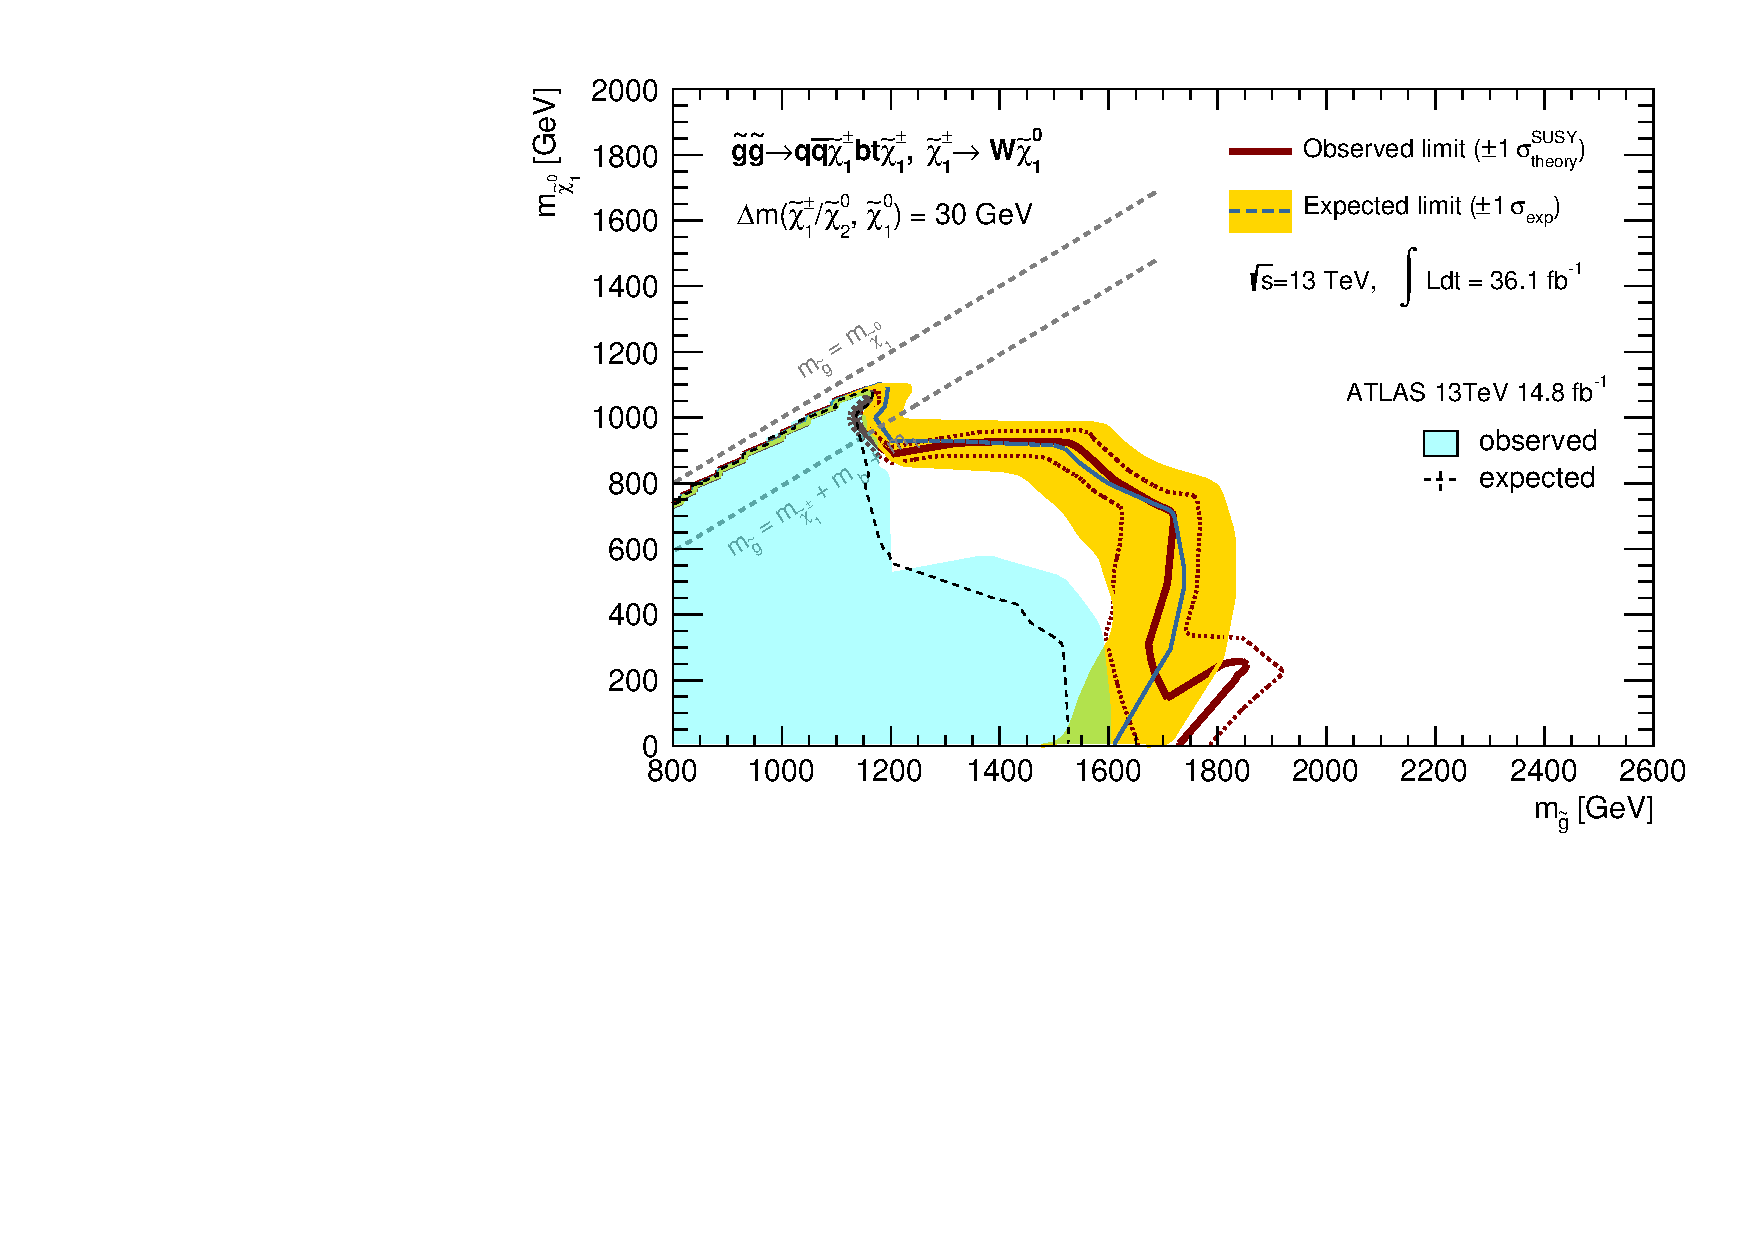
\includegraphics[width=0.48\textwidth]{figures/Result/exclContour/atlascls_wband1_wfixSigXSecband1_showcms0_myAna_tag858_objRep_shapeSys_excl_GG_QQC1BTC1_fixSigXSecNominal_dM30_hypotest__1_harvest_list.pdf}}
    \caption{Projected exlusion limit (95$\%$ CL) for benchmark model \textbf{QQC1BTC1} presented in (a) \xhalf (b) \varx (c) \DMtw (d) \DMth. Observed limit is shown by the solid red line, while the expected limit are expressed by the dashed blue line with the yellow band describing the variation due to the deviation within $\pm1\sigma$. All limits correspond to 95$\%$ CL.
\label{fig::Result::exclLimit::GG_QQC1BTC1} }
\end{figure}

%% --
\begin{figure}
  \begin{center}
    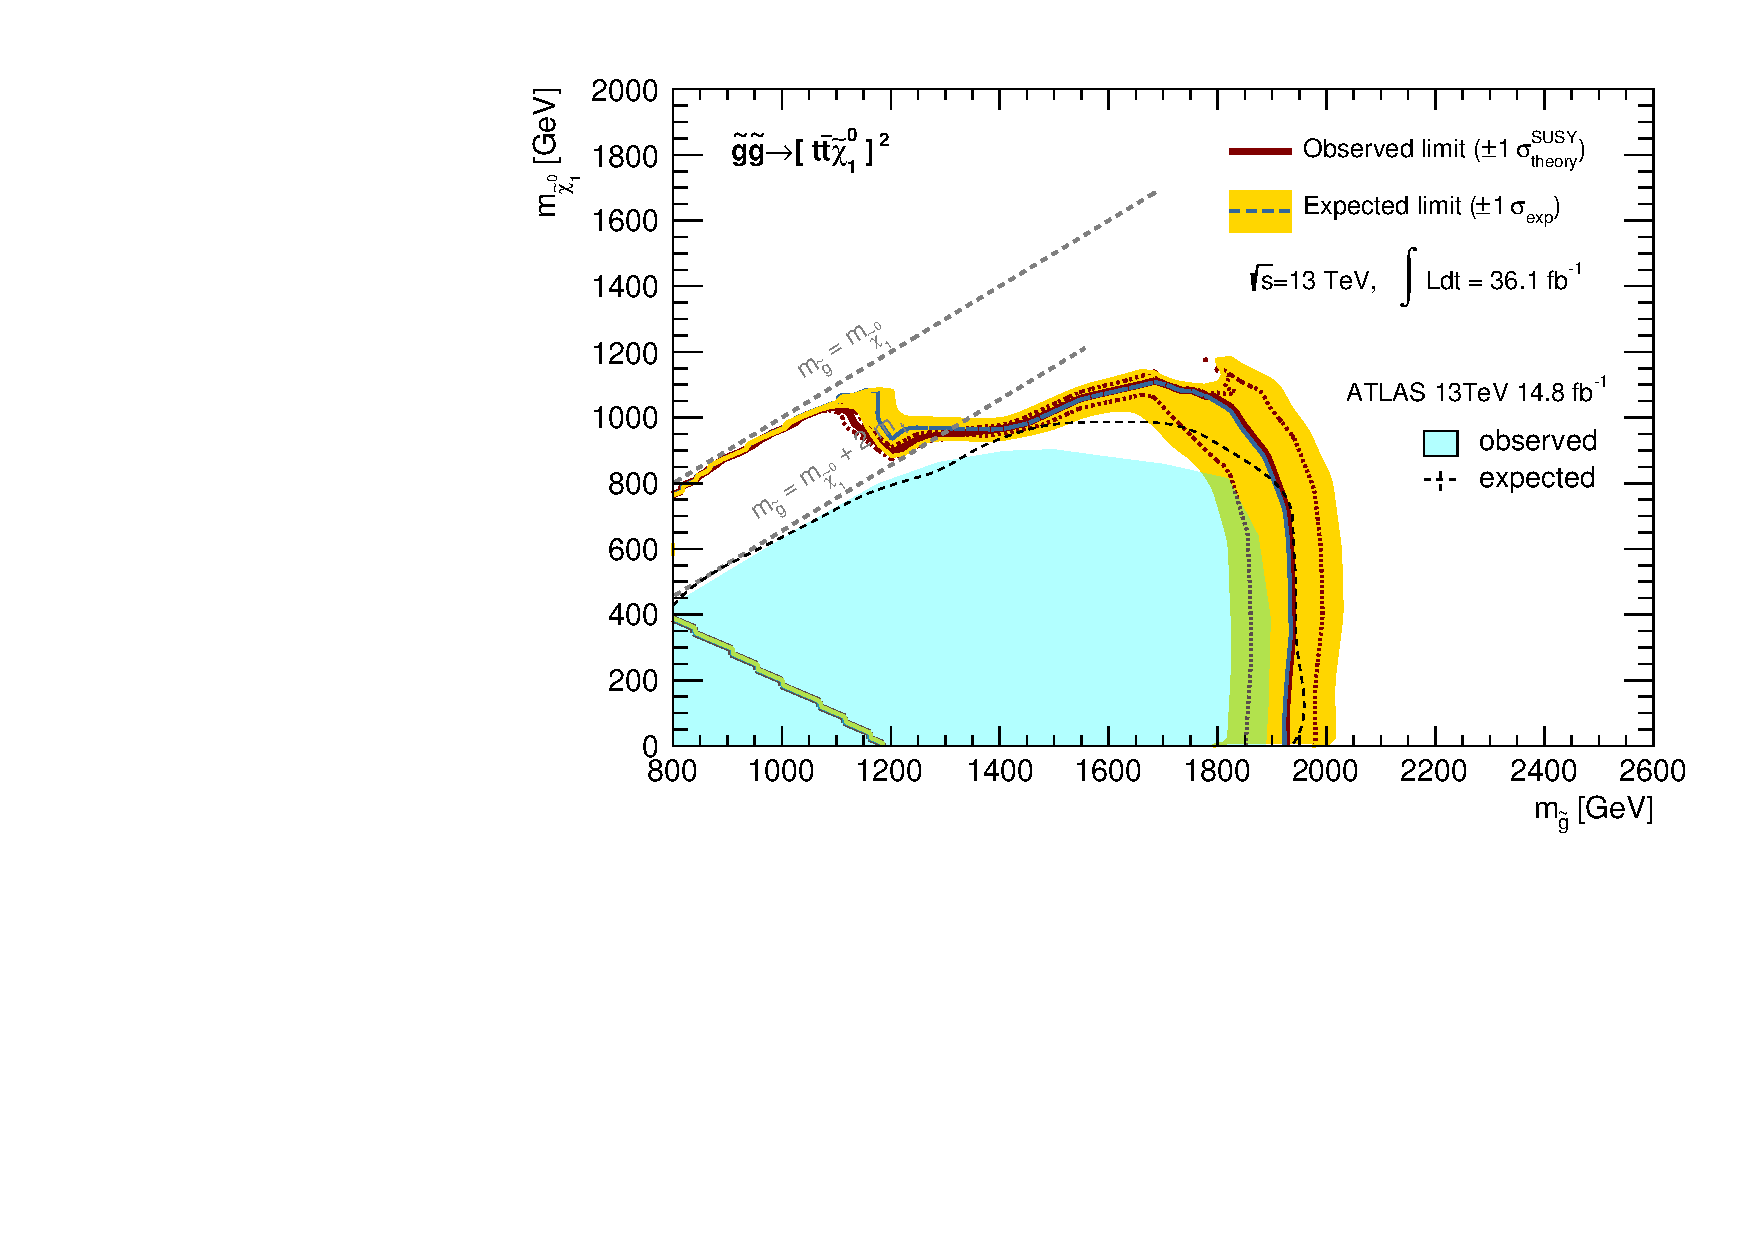
\includegraphics[width=140mm]{figures/Result/exclContour/atlascls_wband1_wfixSigXSecband1_showcms0_myAna_tag858_objRep_shapeSys_excl_GG_symTTN1_fixSigXSecNominal_x12_hypotest__1_harvest_list.pdf}
    \captionof{figure}{Exlusion limit for benchmark model \textbf{TTN1TTN1}.
      Observed limit is shown by the solid red line, while the expected limit are expressed by the dashed blue line with the yellow band describing the variation due to the deviation within $\pm1\sigma$. The up-to-date published result provided by ATLAS \cite{strong3B_ICHEP2016_CONF} is overlaid (observed limit: grey shade, expected limit: black dashed line), which is given by the combination of 0-lepton and 1-lepton analyses. All limits correspond to 95$\%$ CL.
}
    \label{fig::Result::exclLimit::GG_ttn1}
  \end{center}
\end{figure}
%-------------------------------                                                                                                                                                                     




%%%%%%%%%

The exclusion limits for all the 45 models and grids are calculated similarly. Observed limits are compared in Fig. \ref{fig::Result::combLimit::BV1}-\ref{fig::Result::combLimit::3B2}. Models in the same BV/BT/3B type (defined by the different tables in Tab. \ref{tab::Introduction::modelsBV} - \ref{tab::Introduction::models3B}) are overlaid in the same plot. Though the acceptance after the 1-lepton pre-selection are all similar between them, the final seinsitivity does vary depending on the branching into 1-lepton final state of the model, which has relatively a wide variety. This ends up in $300\gev\sim400\gev$ of differece in gluino mass at the worse case. Aside such several models with small 1-lepton branches, the variation is typically $100\gev\sim200\gev$, which indicates inclusive acceptance by the analysis.


%%%%%%%%
%\clearpage
%-------------------------------
\begin{figure}[h]
  \centering
    \subfig{0.49}{figures/Result/combLimit/BV_x12_obs.pdf}{}
    \subfig{0.49}{figures/Result/combLimit/BV_varx_obs.pdf}{}
    \subfig{0.49}{figures/Result/combLimit/BV_dM20_obs.pdf}{}
    \subfig{0.49}{figures/Result/combLimit/BV_dM30_obs.pdf}{}
    \caption{
    Observed limit for BV benchmark moelds (defined in Table \ref{tab::Introduction::modelsBV}) presented in grid (a) $\xhalf$ (b) $\varx$ (c) $\DMtw$ (d) $\DMth$.
      \label{fig::Result::combLimit::BV1} }
\end{figure}
%-------------------------------


\clearpage
%-------------------------------
\begin{figure}[h]
  \centering
    \subfig{0.9}{figures/Result/combLimit/BT_x12_obs.pdf}{}
    \subfig{0.9}{figures/Result/combLimit/BT_varx_obs.pdf}{}
    \caption{
    Observed limit for BT benchmark models (defined in Table \ref{tab::Introduction::modelsBT}) presented in grid (a) $\xhalf$ (b) $\varx$.
      \label{fig::Result::combLimit::BT1} }
\end{figure}


\begin{figure}[h]
  \centering
    \subfig{0.9}{figures/Result/combLimit/BT_dM20_obs.pdf}{}
    \subfig{0.9}{figures/Result/combLimit/BT_dM30_obs.pdf}{}
    \caption{
    Observed limit for BT benchmark models (defined in Table \ref{tab::Introduction::modelsBT}) presented in grid (a) $\DMtw$ (b) $\DMth$.
      \label{fig::Result::combLimit::BT2} }
\end{figure}
%-------------------------------



\clearpage
%-------------------------------
\begin{figure}[h]
  \centering
    \subfig{0.9}{figures/Result/combLimit/3B_x12_obs.pdf}{}
    \subfig{0.9}{figures/Result/combLimit/3B_varx_obs.pdf}{}
    \caption{
    Observed limit for 3B benchmark models (defined in Table \ref{tab::Introduction::models3B}) presented in grid (a) $\xhalf$ (b) $\varx$.
      \label{fig::Result::combLimit::3B1} }
\end{figure}

\begin{figure}[h]
  \centering
    \subfig{0.9}{figures/Result/combLimit/3B_dM20_obs.pdf}{}
    \subfig{0.9}{figures/Result/combLimit/3B_dM30_obs.pdf}{}
    \caption{
    Observed limit for 3B benchmark models (defined in Table \ref{tab::Introduction::models3B}) presented in grid (a) $\DMtw$ (b) $\DMth$.
      \label{fig::Result::combLimit::3B2} }
\end{figure}
%-------------------------------




%%%%%%%

\clearpage
\subsubsection{Cross-section Upper limit}
In a hypothetical test, the $\mathrm{CL_s}$ values are calculated for multiple points in $\mu_{\mathrm{sig.}}$, ranging from $0\sim10$. $\mathrm{CL_s}$ is then modeled as funtion of $\mu_{\mathrm{sig.}}$, therefore the upper limit on $\mu_{\mathrm{sig.}}$ can be defined by:
$$
\mu_{\mathrm{sig.},95} := \mu_{\mathrm{sig.}}(\mathrm{CL_s}=0.05),
$$
for each signal points in the model.
This can be straightforwardly interpreted into cross-section upper limit ($\sigma_{95}$), which can be model-independenly ultimately by computing $\sigma_{95}$ as the function of masses of gluino and EW-gauginos including the LSP, for all the decay model of gluino. Fig. \ref{fig::Result::xsecUL::QQC1QQC1}-Fig. \ref{fig::Result::xsecUL::TTN1TTN1} present the results for the reference models QQC1QQC1, QQC1BTC1 and TTN1TTN1.
%, and the full result are in the Appendix \ref{sec::Result::xsecUL::nonBenchMark}.


\clearpage
%% -- xsec UL ----------------------
\begin{figure}[h]
  \centering
%    \subfigure[]{\includegraphics[width=0.48\textwidth]{figures/Result/xsecUL/onestepCC_x12.pdf}}
%    \subfigure[]{\includegraphics[width=0.48\textwidth]{figures/Result/xsecUL/onestepCC_varx.pdf}}
    \subfigure[]{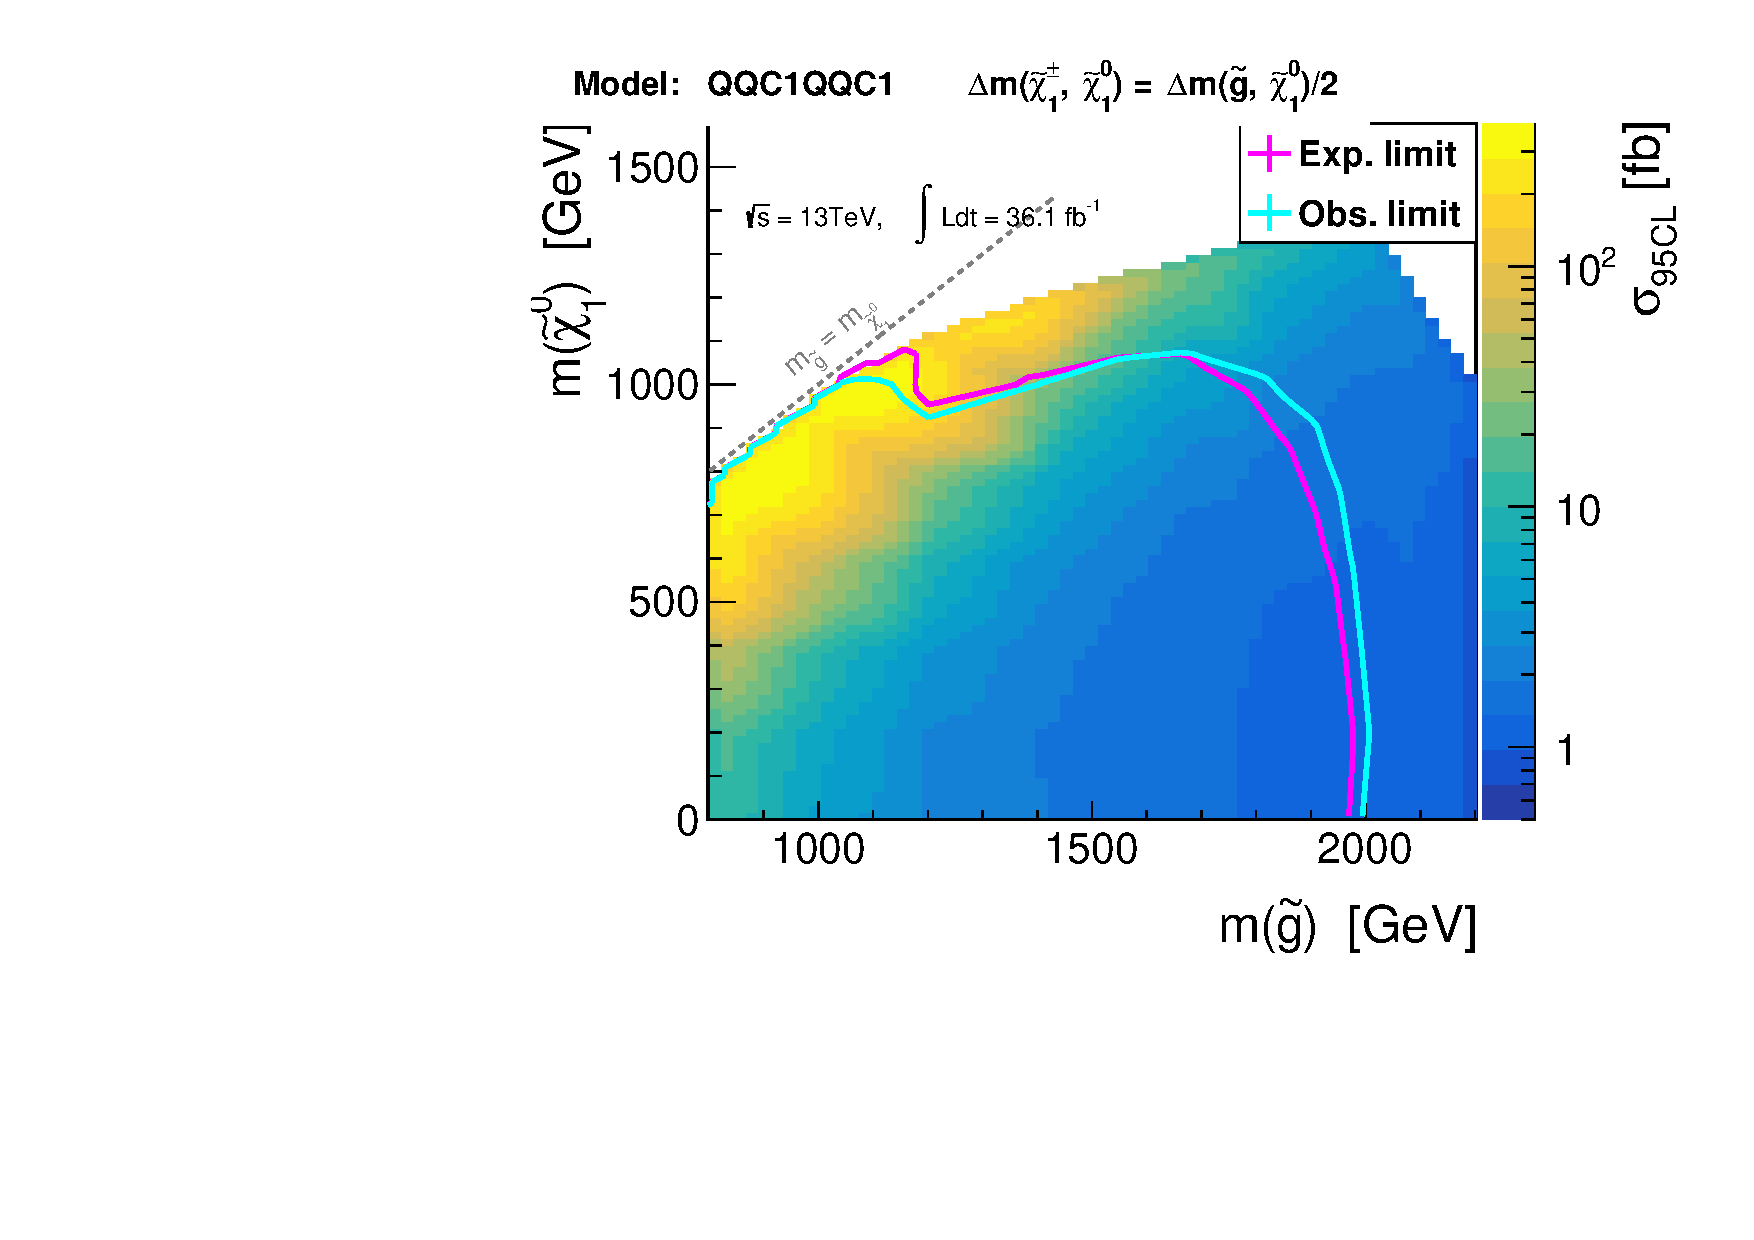
\includegraphics[width=0.48\textwidth]{figures/Result/xsecUL/symQQC1_x12.pdf}}
    \subfigure[]{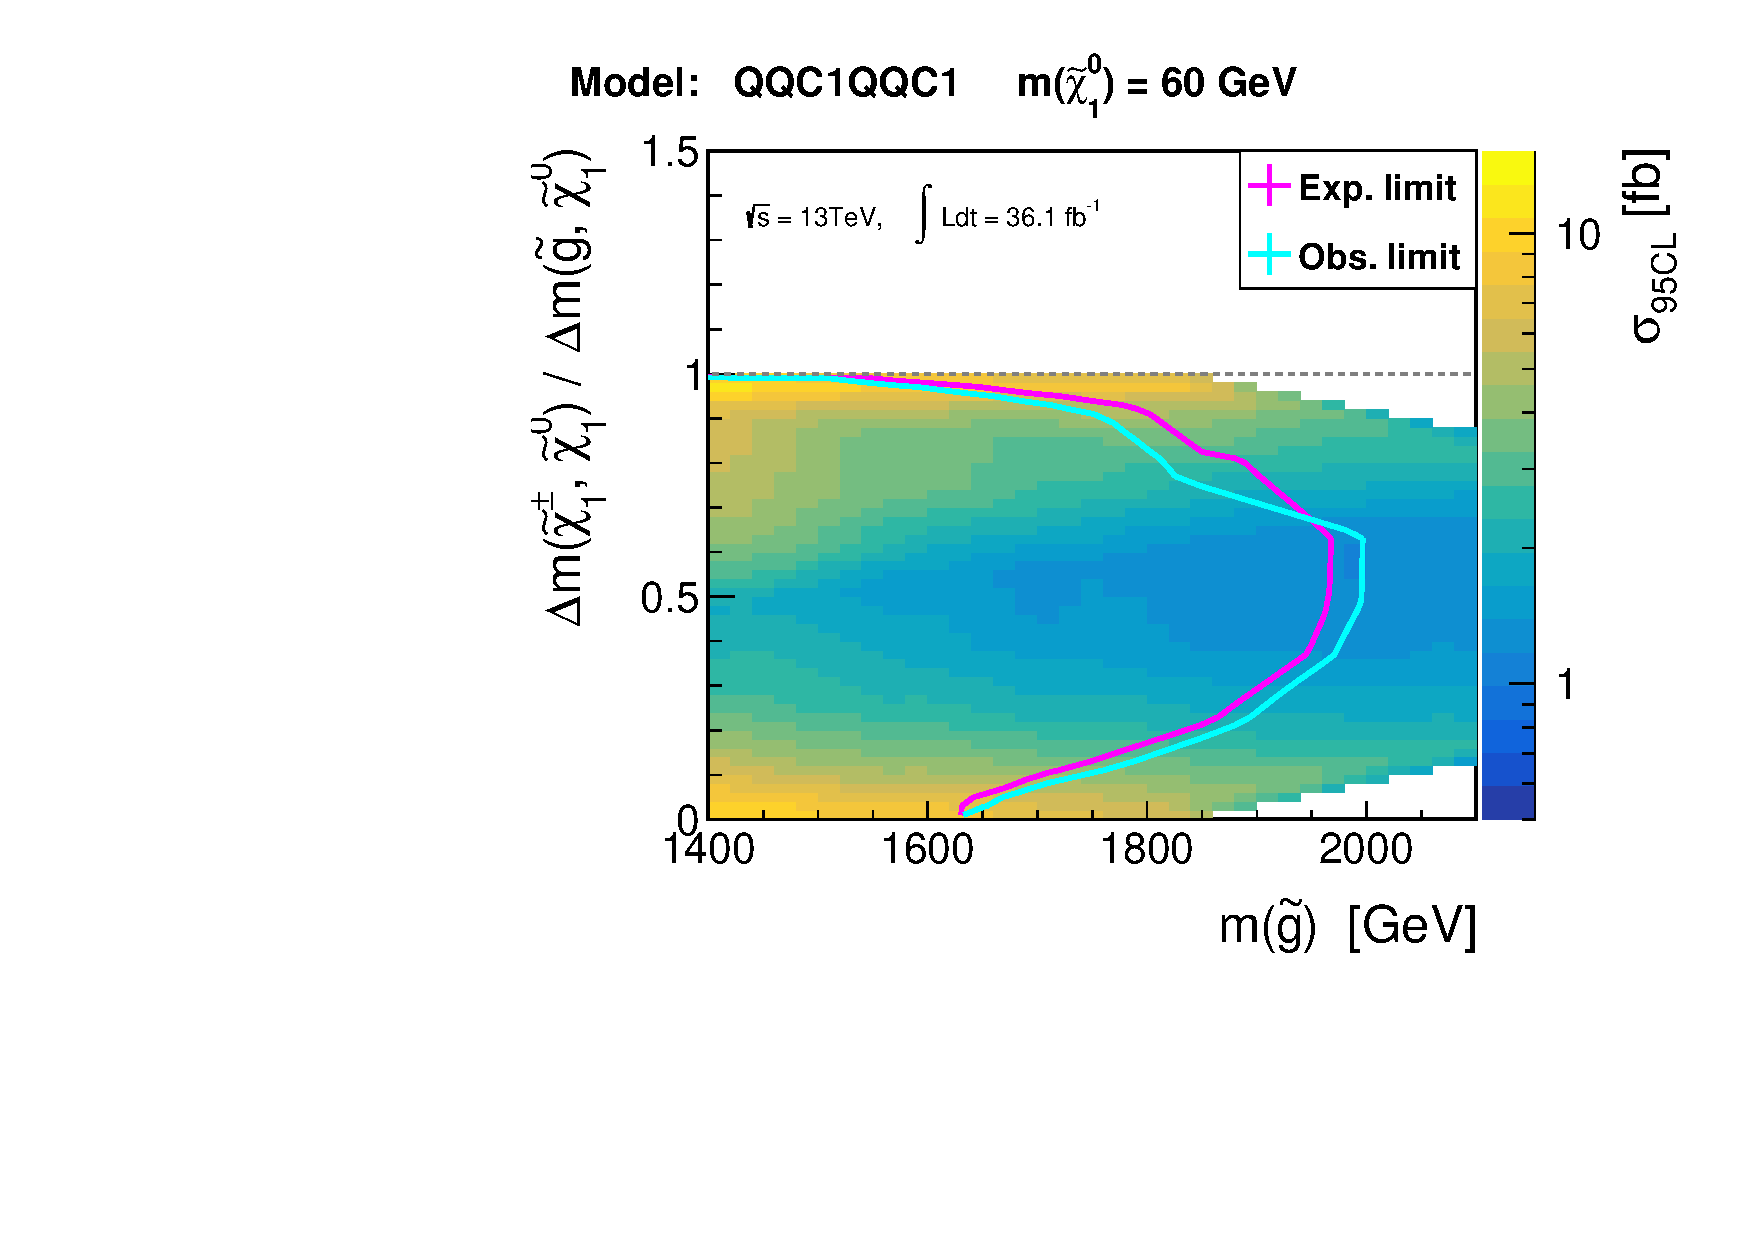
\includegraphics[width=0.48\textwidth]{figures/Result/xsecUL/symQQC1_varx.pdf}}
    \subfigure[]{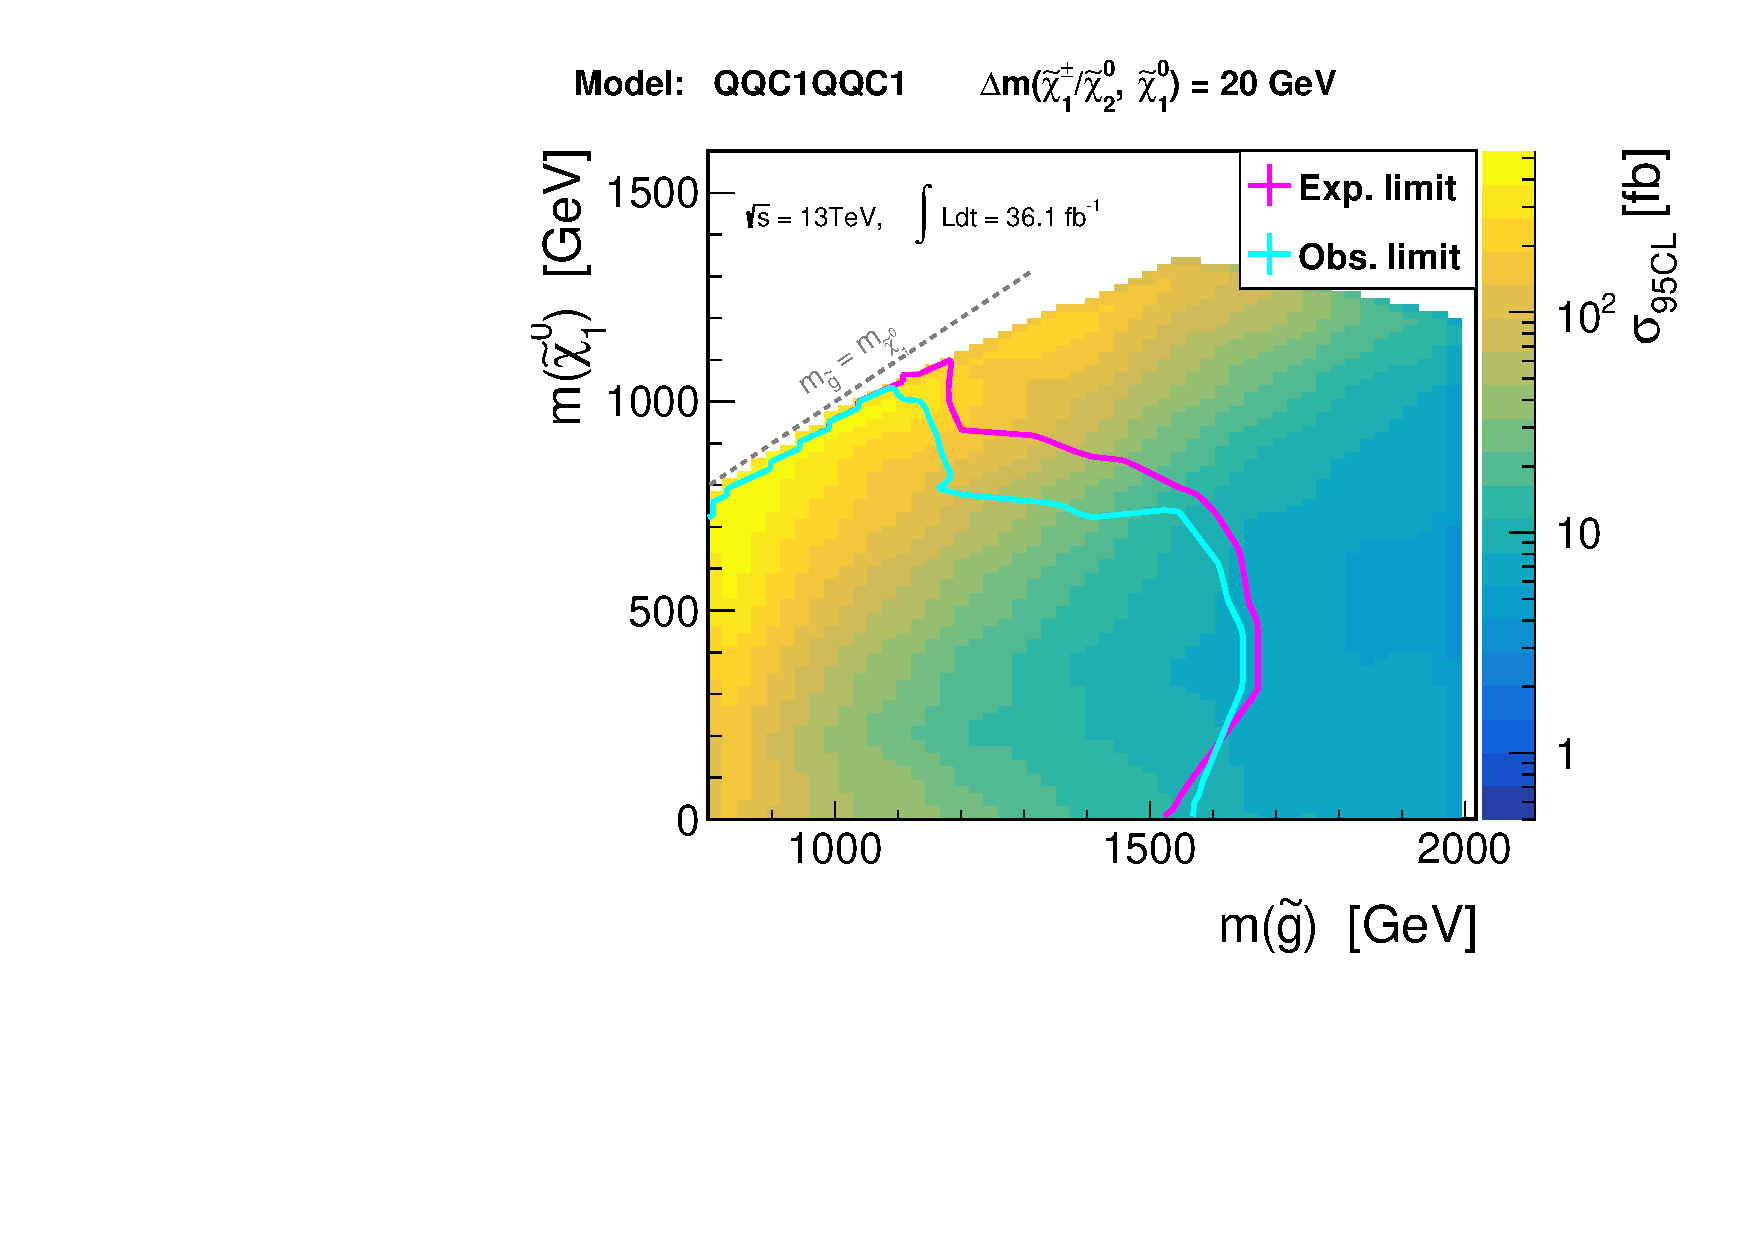
\includegraphics[width=0.48\textwidth]{figures/Result/xsecUL/symQQC1_dM20.pdf}}
    \subfigure[]{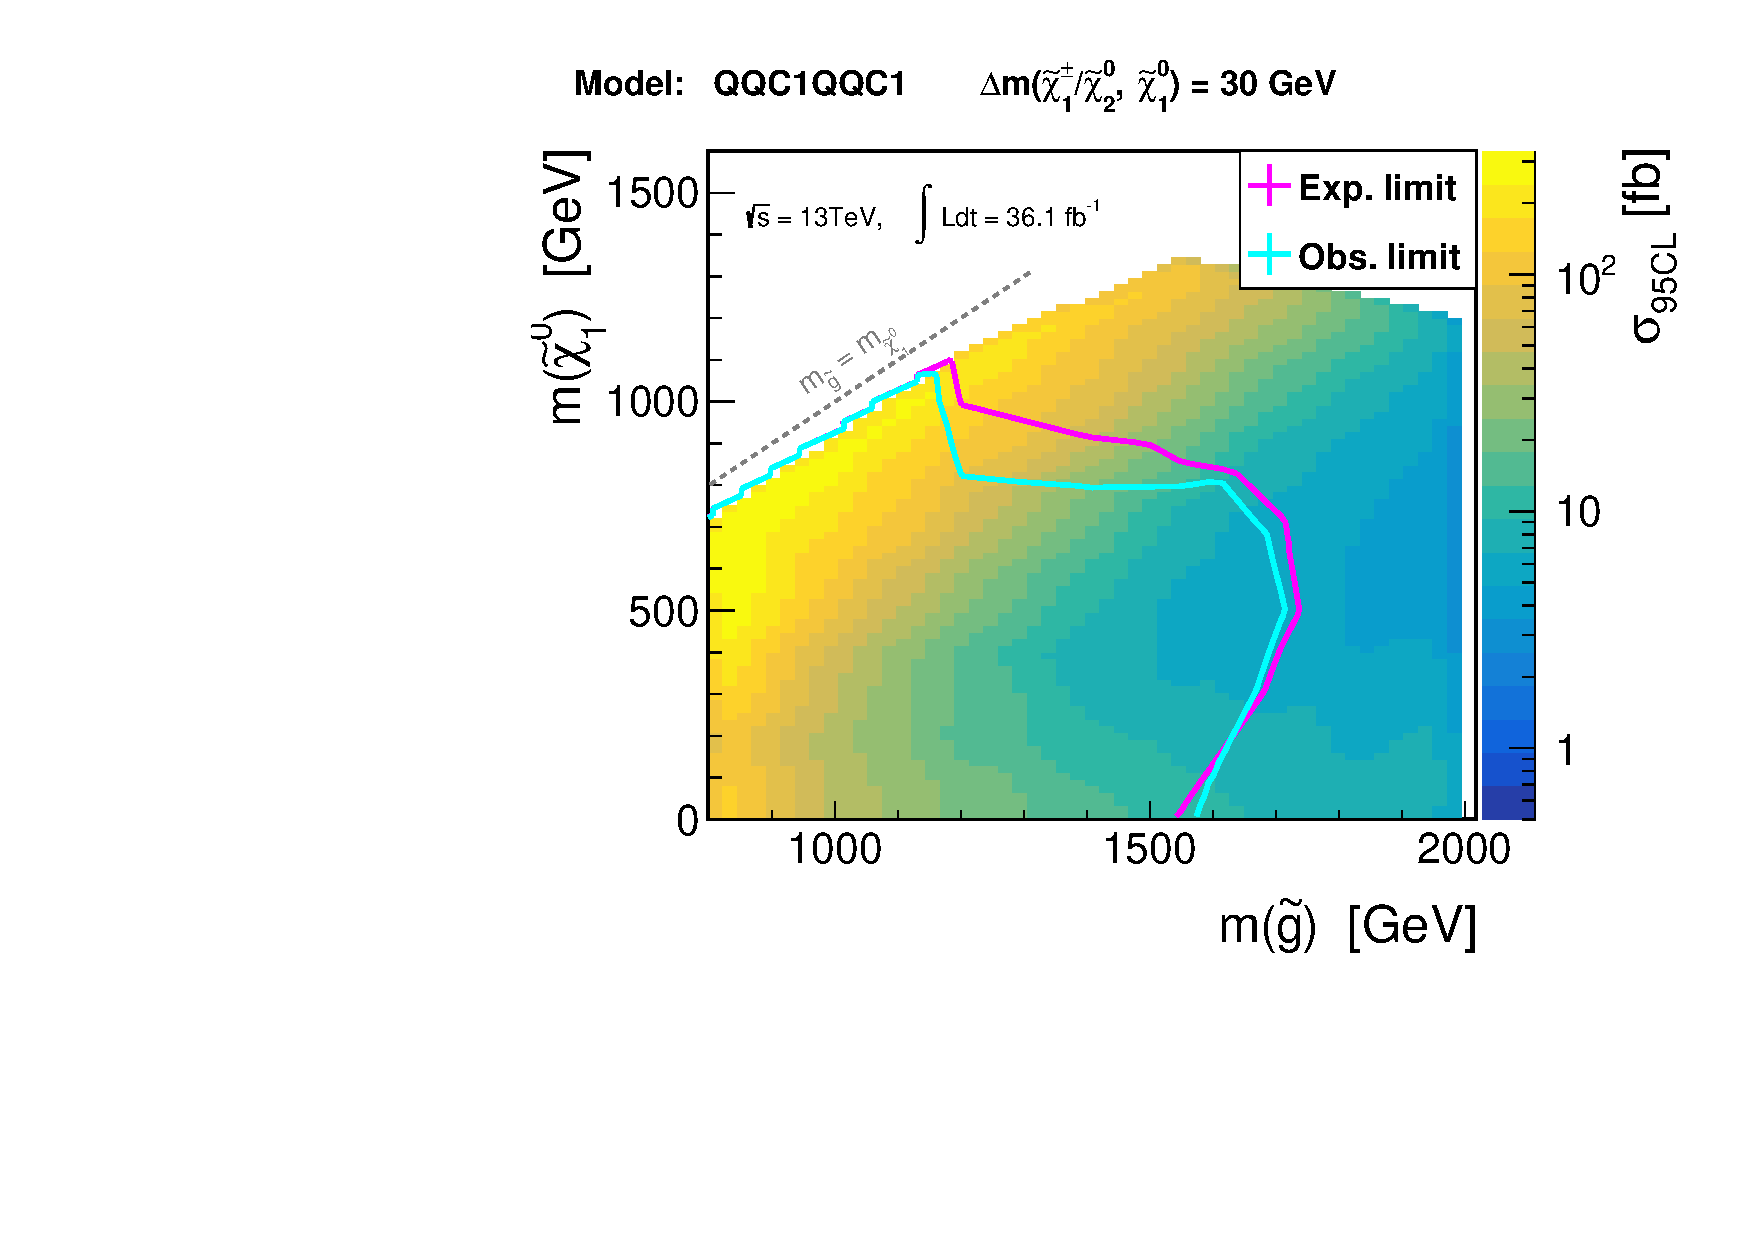
\includegraphics[width=0.48\textwidth]{figures/Result/xsecUL/symQQC1_dM30.pdf}}
    \caption{
    Upper limit of excluded cross-section (95$\%$CL) as the function of the SUSY masses, for benchmark model \textbf{QQC1QQC1}, presented in the grids (a) $x=1/2$ (b) $\mLSP=60\gev$ (c) $\dmc=20\gev$ (d) $\dmc=30\gev$.
    \label{fig::Result::xsecUL::QQC1QQC1} }
\end{figure}


%figures/Result/xsecUL/symQQC1_dM20.pdf

%% --
\begin{figure}[h]
  \centering
    \subfigure[]{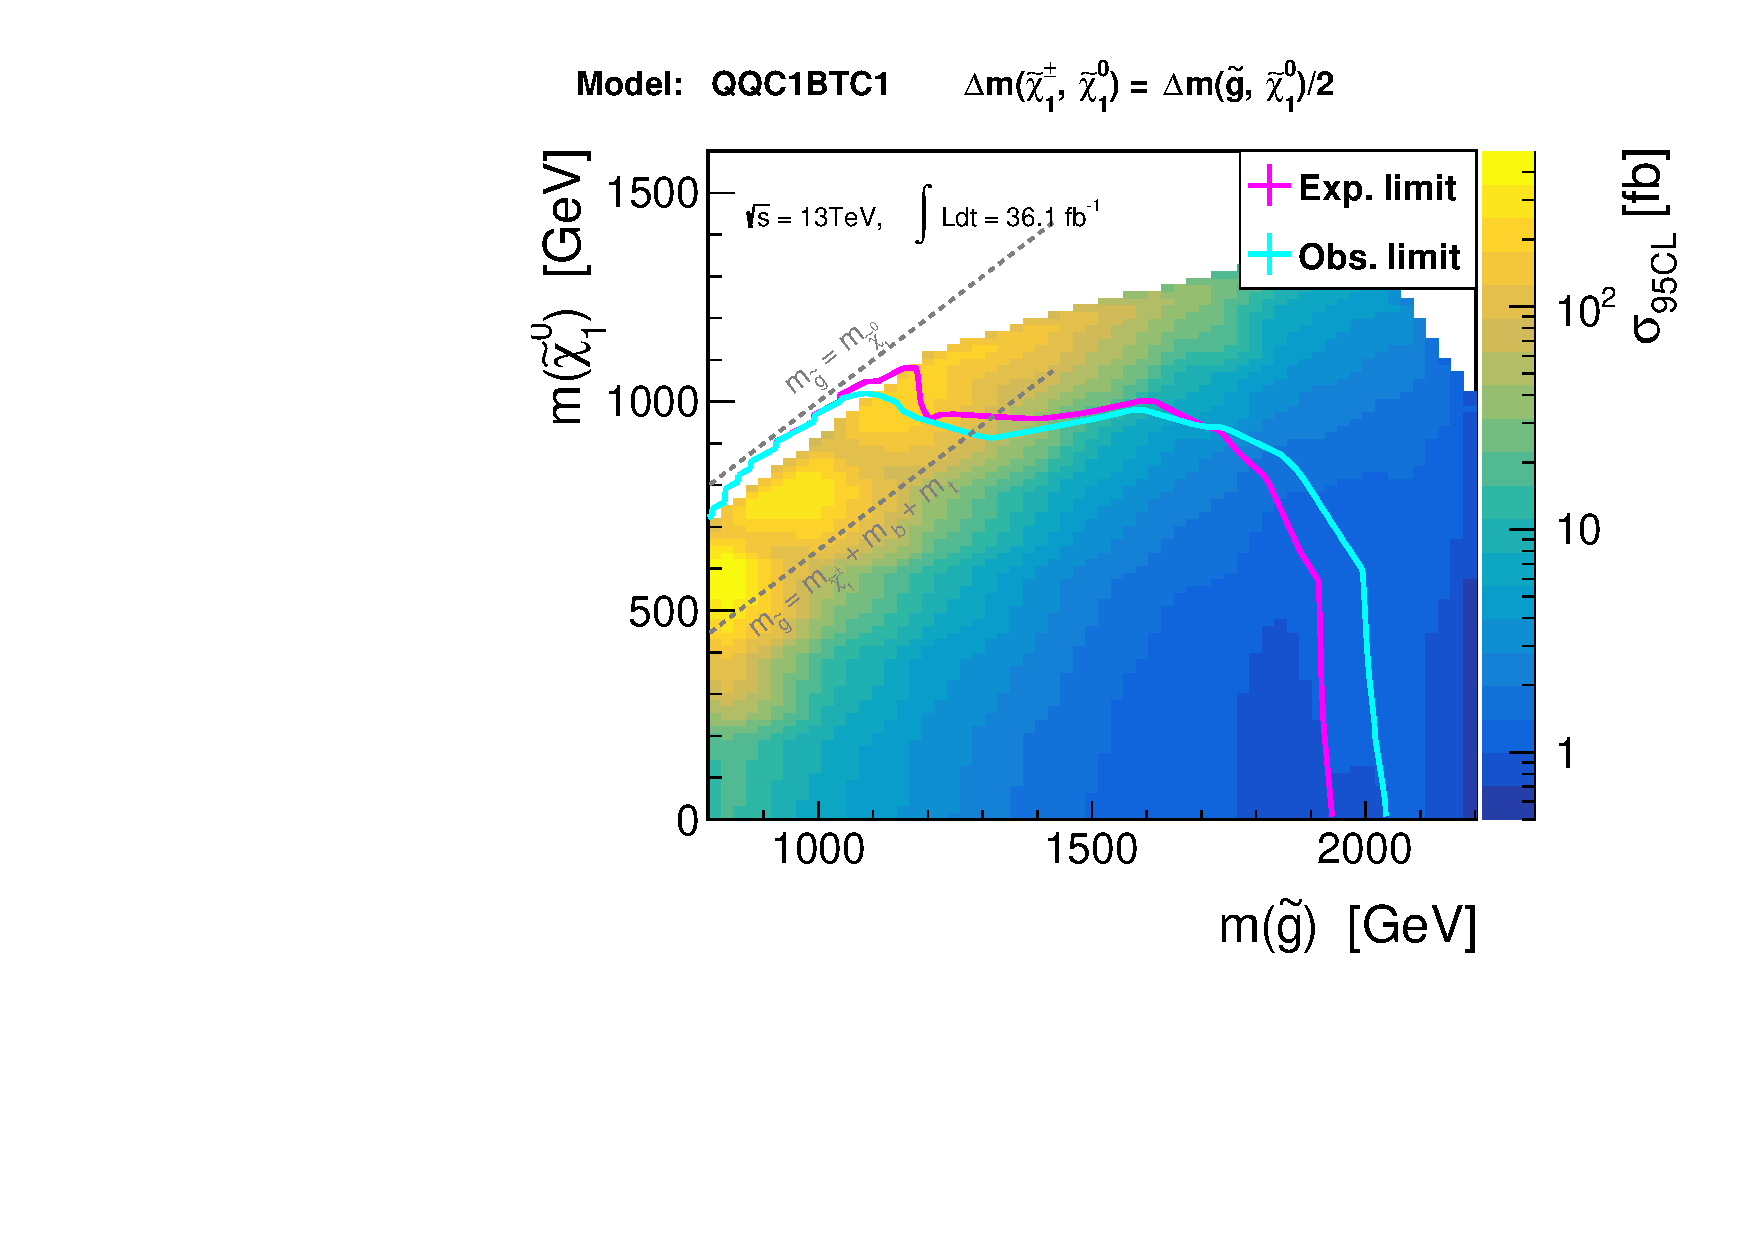
\includegraphics[width=0.48\textwidth]{figures/Result/xsecUL/QQC1BTC1_x12.pdf}}
    \subfigure[]{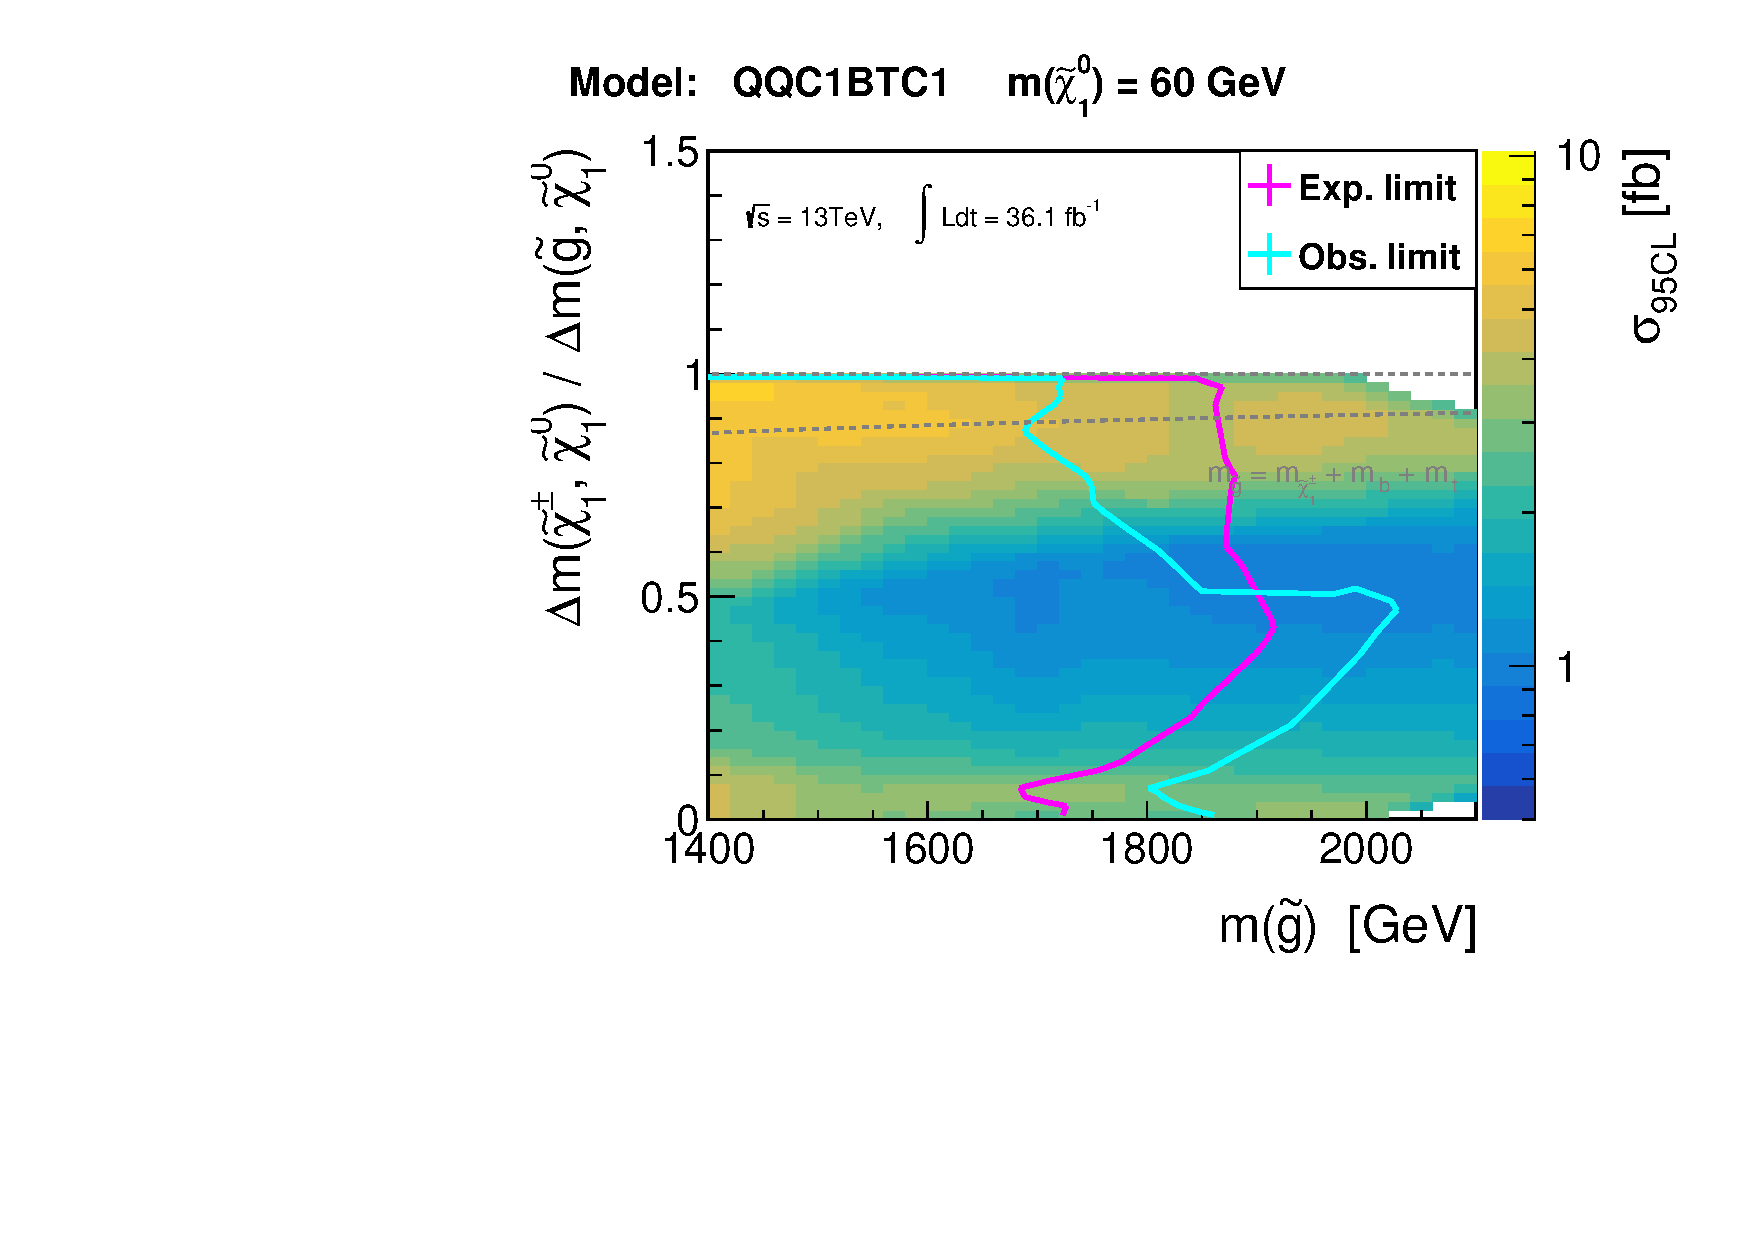
\includegraphics[width=0.48\textwidth]{figures/Result/xsecUL/QQC1BTC1_varx.pdf}}
    \subfigure[]{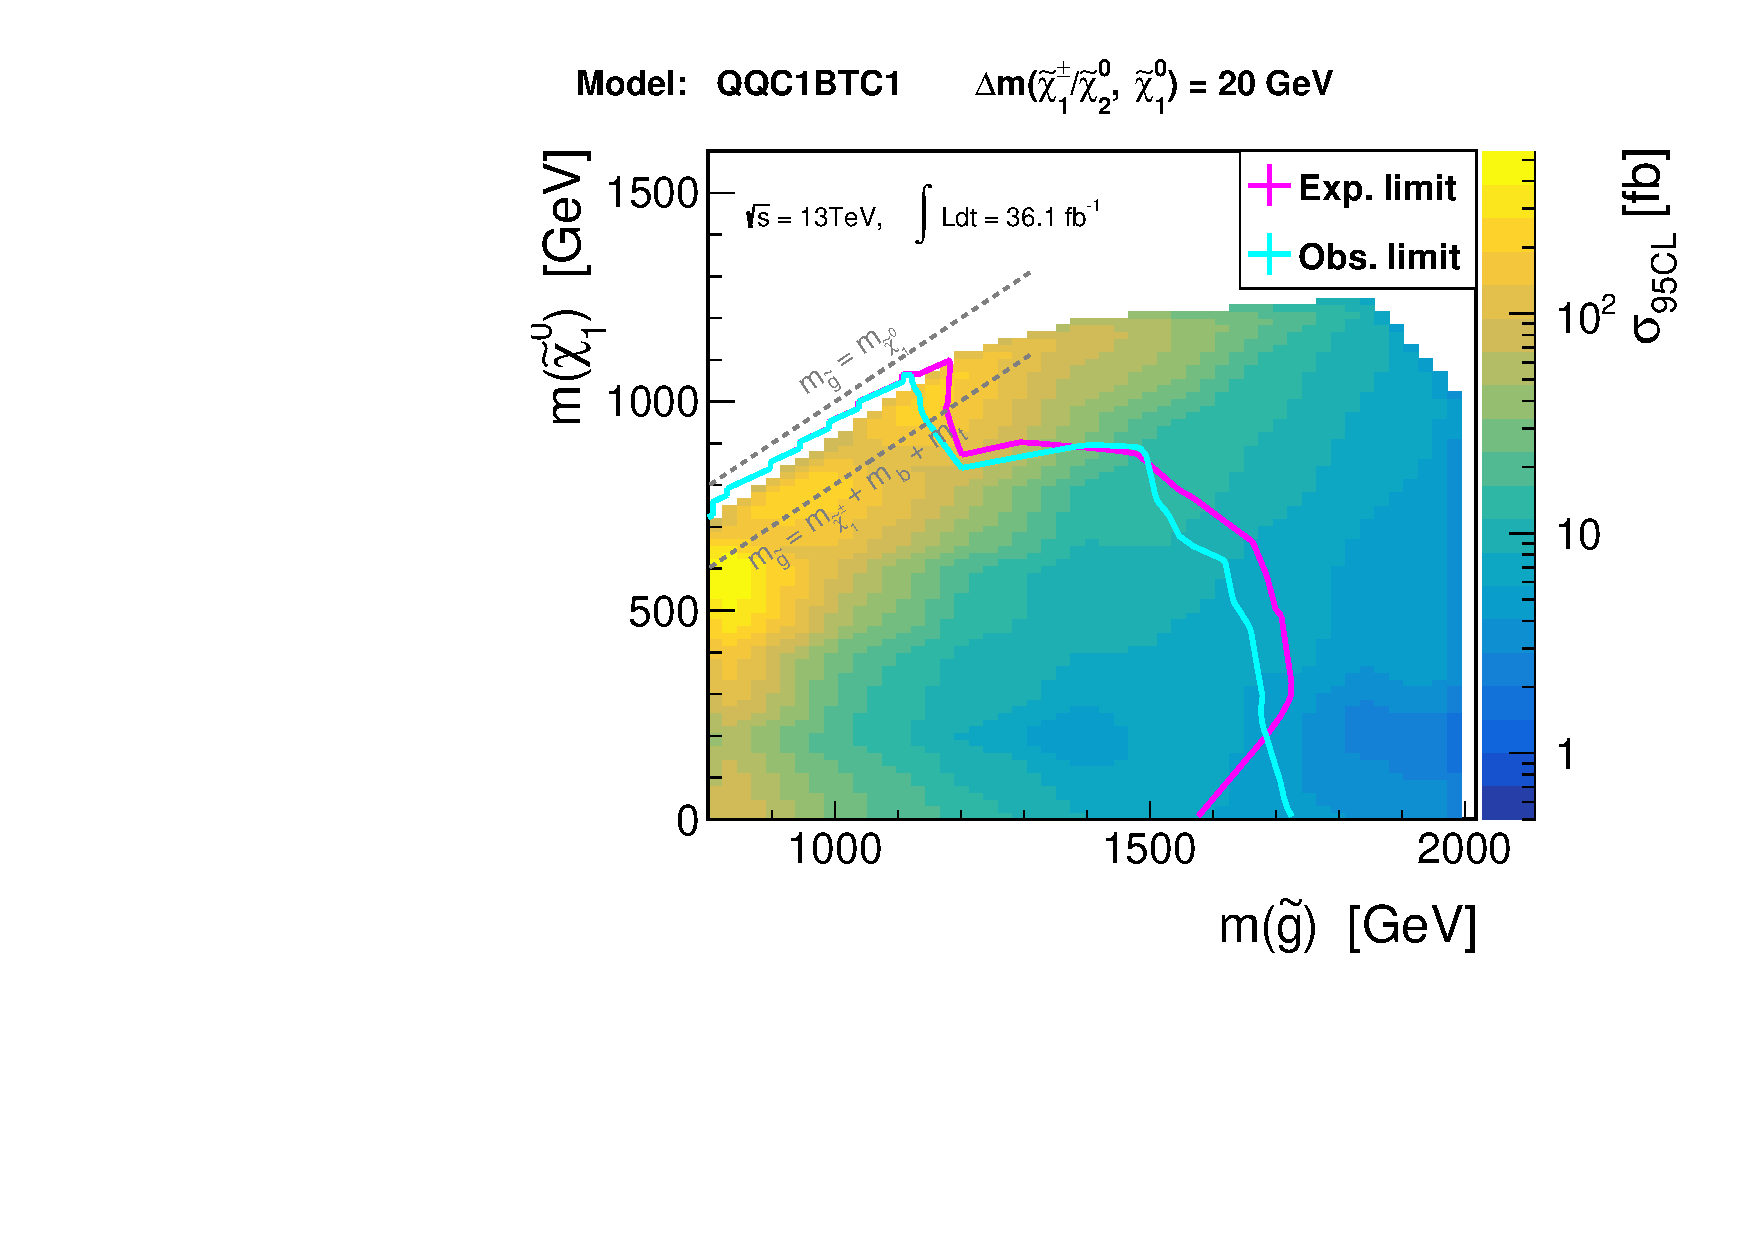
\includegraphics[width=0.48\textwidth]{figures/Result/xsecUL/QQC1BTC1_dM20.pdf}}
    \subfigure[]{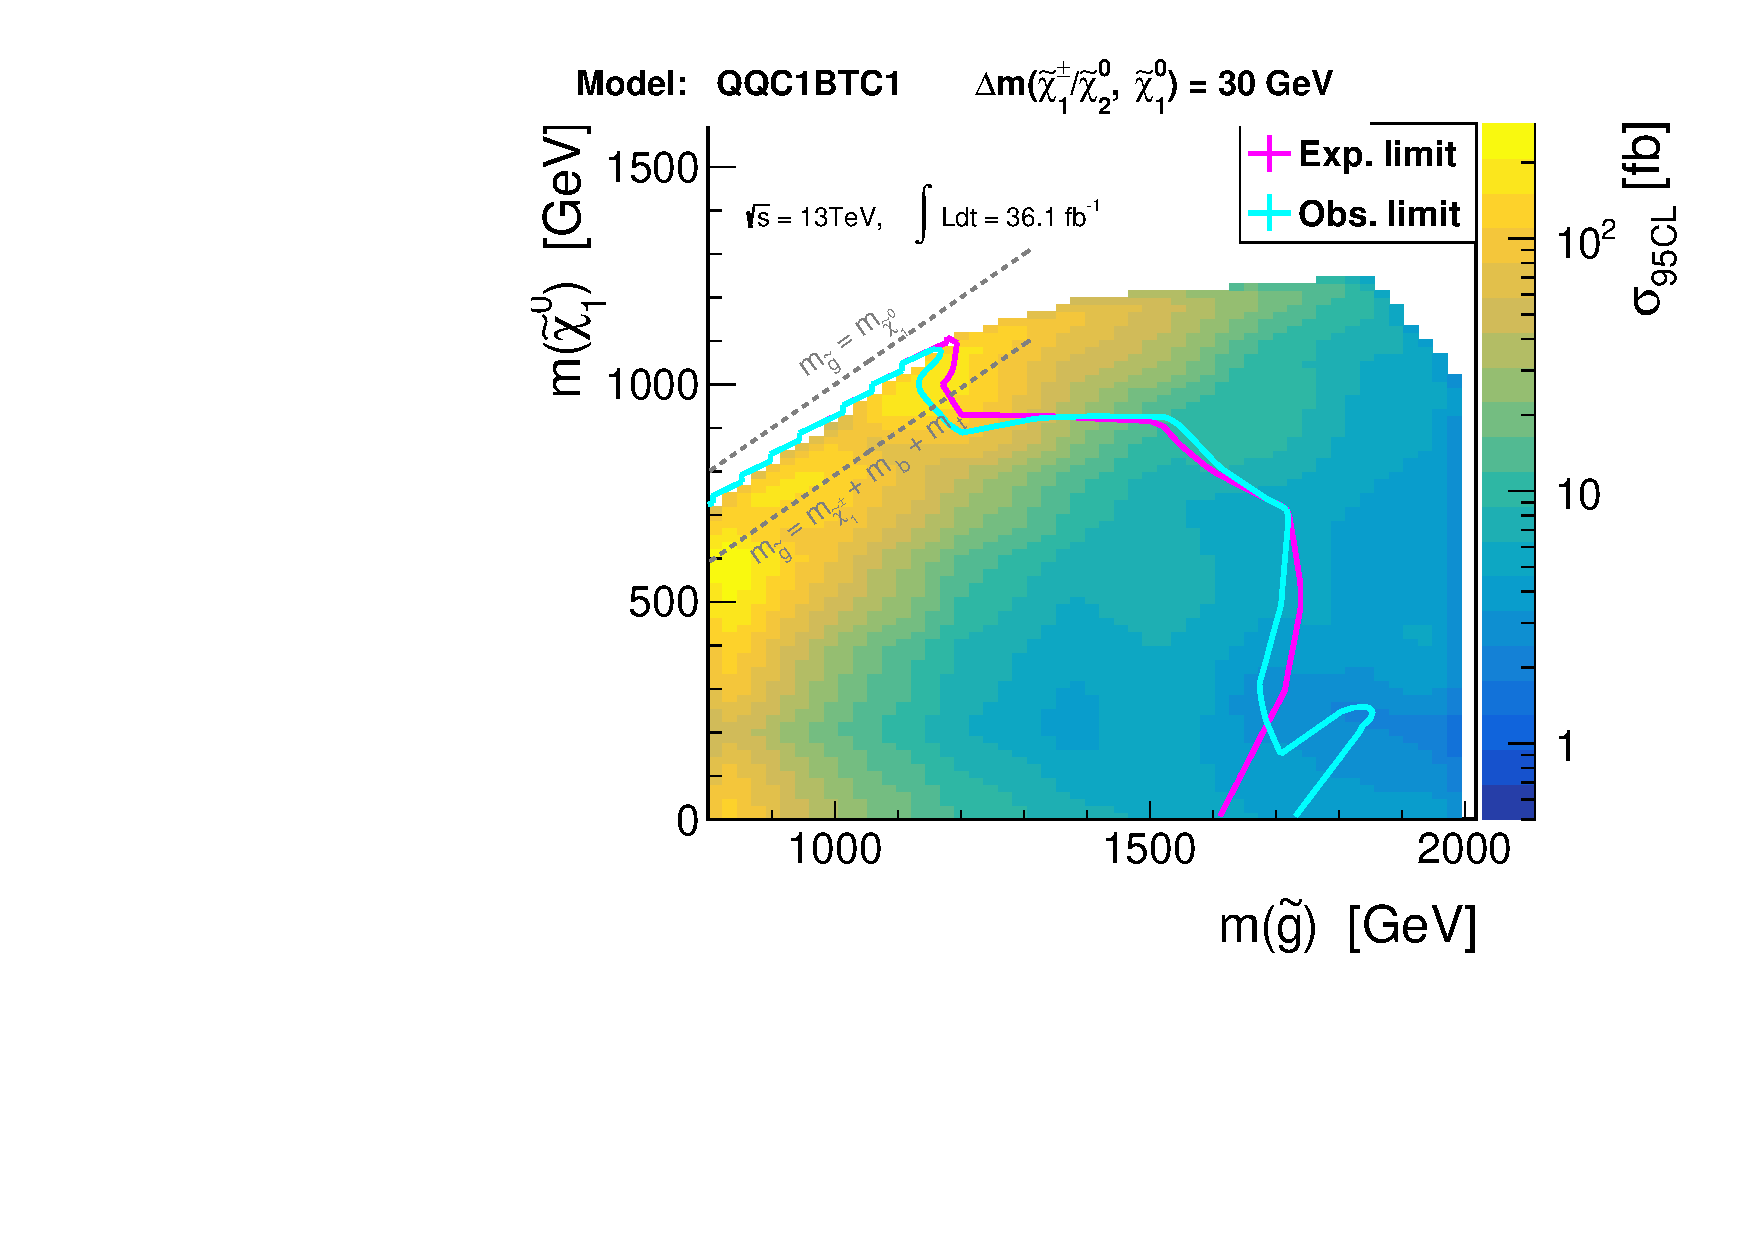
\includegraphics[width=0.48\textwidth]{figures/Result/xsecUL/QQC1BTC1_dM30.pdf}}
    \caption{
    Upper limit of excluded cross-section (95$\%$CL) as the function of the SUSY masses, for benchmark model \textbf{QQC1BTC1}, presented in the grids (a) $x=1/2$ (b) $\mLSP=60\gev$ (c) $\dmc=20\gev$ (d) $\dmc=30\gev$.
    \label{fig::Result::xsecUL::QQC1BTC1} }
\end{figure}

%% --
\begin{figure}
  \begin{center}
    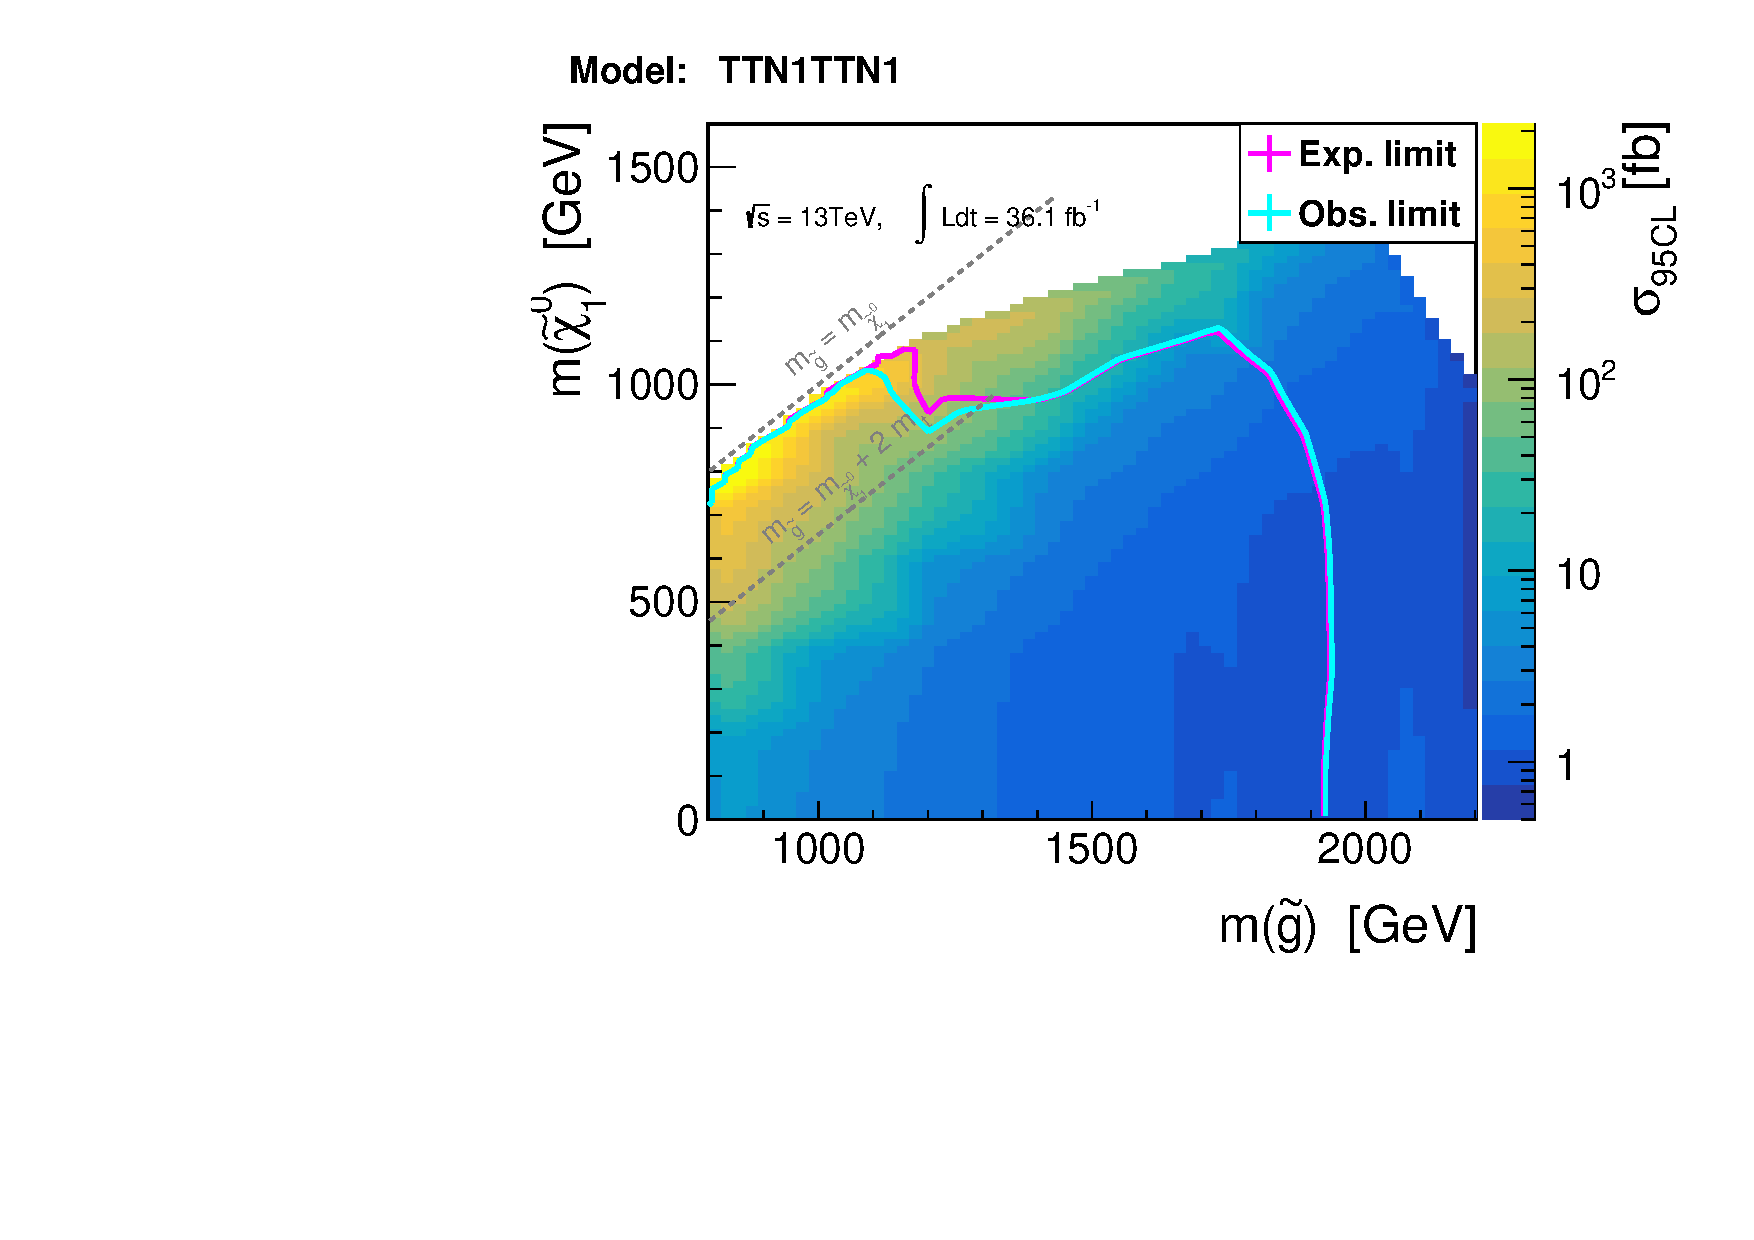
\includegraphics[width=160mm]{figures/Result/xsecUL/symTTN1_x12.pdf}
    \captionof{figure}{
    Upper limit of excluded cross-section (95$\%$CL) as the function of the SUSY masses, for benchmark model
 \textbf{TTN1TTN1}.
    \label{fig::Result::xsecUL::TTN1TTN1} }       
  \end{center}
\end{figure}
%-------------------------------                                                                                                   






%\subsection{Discussion}
